Abaixo seguem os a imagens dos padrões de difração gerados, juntamente com as tabelas de dados calculados a partir das mesmas, além daqueles obtidos com microscópio metrológico.


\subsection{Fendas C}

\DTLloaddb{medidasC}{dados/C.csv}

\begin{table}[H]
	\centering
	\sisetup{
		table-figures-uncertainty = 1,
		zero-decimal-to-integer
	}
	\begin{tabular}{cccccc}
		\toprule\toprule
            \multirow{2}*{\bfseries Fenda}
				& \multirow{2}*{\bfseries $n_y$}
				& \multirow{2}*{\bfseries $n_y \Delta y$ [\si{\milli\meter}]}
				& \multirow{2}*{\bfseries $\Delta y$ [\si{\milli\meter}]}
				& \multicolumn{2}{c}{\bfseries $b$ [\si{\micro\meter}]}
			\\ & & & & Calculado & Microscópio

		\DTLforeach*{medidasC}{\fenda=id,\nDy=nDy,\yr=yr,\n=n,\Dy=Dy,\Dyr=Dyr,\b=b,\br=br,\bm=bm,\bmr=bmr}{
			\DTLiffirstrow{\\\midrule}{\\}
			\fenda
				& $\num{\n}$
				& $\num{\nDy(\yr)}$
				& $\num{\Dy(\Dyr)}$
				& $\num{\b(\br)}$
				& $\num[zero-decimal-to-integer=false]{\bm(\bmr)}$
		}
        \\\bottomrule\bottomrule
	\end{tabular}

	\caption{Dados obtidos para os padrões de difração das fendas da linha C}
	\label{tab:fend_c}
\end{table}
\begin{figure}[H]
    \centering

    \begin{subfigure}[t]{.6\textwidth}
        \centering
        \begingroup
  \sbox{\tempbox}{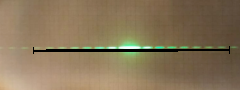
\includegraphics[width=\textwidth]{figuras/medidas/C4.pdf}}
  \begin{picture}(\wd\tempbox,\ht\tempbox)
    \put(0,0){\usebox{\tempbox}}
    \put(.502\wd\tempbox,.33\ht\tempbox){$8~\Delta y$}
  \end{picture}
\endgroup


        \caption{C4}
        \label{fig:C4}
    \end{subfigure}
    \qquad
    \begin{subfigure}[t]{.6\textwidth}
        \centering
        \begingroup
  \sbox{\tempbox}{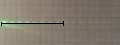
\includegraphics[width=\textwidth]{figuras/medidas/C5.pdf}}
  \begin{picture}(\wd\tempbox,\ht\tempbox)
    \put(0,0){\usebox{\tempbox}}
    \put(.22\wd\tempbox,.38\ht\tempbox){$4~\Delta y$}
  \end{picture}
\endgroup


        \caption{C5}
        \label{fig:C5}
    \end{subfigure}
    \qquad
    \begin{subfigure}[t]{.6\textwidth}
        \centering
        \begingroup
  \sbox{\tempbox}{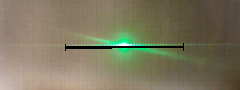
\includegraphics[width=\textwidth]{figuras/medidas/C6.pdf}}
  \begin{picture}(\wd\tempbox,\ht\tempbox)
    \put(0,0){\usebox{\tempbox}}
    \put(.47\wd\tempbox,.39\ht\tempbox){$20~\Delta y$}
  \end{picture}
\endgroup


        \caption{C6}
        \label{fig:C6}
    \end{subfigure}

    \caption{Fotos dos padrões de difração das fendas C}
    \label{fig:C}
\end{figure}

\subsection{Fendas B}

\DTLloaddb{medidasB}{dados/B.csv}

\begin{table}[H]
	\centering
	\sisetup{
		table-figures-uncertainty = 1,
		zero-decimal-to-integer
	}
	\begin{tabular}{ccccccc}
		\toprule\toprule
            {\bfseries Fenda}
				& {\bfseries $n_y$}
				& {\bfseries $n_y \Delta y$ [\si{\milli\meter}]}
				& {\bfseries $\Delta y$ [\si{\milli\meter}]}
				& {\bfseries $n_\Lambda$}
				& {\bfseries $n_\Lambda \Lambda$ [\si{\milli\meter}]}
				& {\bfseries $\Lambda$ [\si{\milli\meter}]}

		\DTLforeach*{medidasB}{\fenda=id,\nDy=nDy,\yr=yr,\n=n,\Dy=Dy,\Dyr=Dyr,\mL=mL,\m=m,\L=L,\Lr=Lr,\b=b,\br=br,\h=h,\hr=hr,\bm=bm,\hm=hm,\ymr=ymr}{
			\DTLiffirstrow{\\\midrule}{\\}
			\fenda
				& $\num{\n}$
				& $\num{\nDy(\yr)}$
				& $\num{\Dy(\Dyr)}$
				& $\num{\m}$
				& $\num{\mL(\yr)}$
				& $\num{\L(\Lr)}$
		}
        \\\bottomrule\bottomrule
	\end{tabular}

	\caption{Dados obtidos para os padrões de difração das fendas da linha B}
	\label{tab:fend_b1}
\end{table}
\begin{table}[H]
	\centering
	\sisetup{
		table-figures-uncertainty = 1,
		zero-decimal-to-integer
	}
	\begin{tabular}{ccccc}
		\toprule\toprule
            \multirow{2}*{\bfseries Fenda}
				& \multicolumn{2}{c}{\bfseries $b$ [\si{\micro\meter}]}
				& \multicolumn{2}{c}{\bfseries $h$ [\si{\micro\meter}]}
			\\ & Calculado & Microscópio & Calculado & Microscópio

		\DTLforeach*{medidasB}{\fenda=id,\nDy=nDy,\yr=yr,\n=n,\Dy=Dy,\Dyr=Dyr,\mL=mL,\m=m,\L=L,\Lr=Lr,\b=b,\br=br,\h=h,\hr=hr,\bm=bm,\hm=hm,\ymr=ymr}{
			\DTLiffirstrow{\\\midrule}{\\}
			\fenda
				& $\num{\b(\br)}$
				& $\num[zero-decimal-to-integer=false]{\bm(\ymr)}$
				& $\num{\h(\hr)}$
				& $\num[zero-decimal-to-integer=false]{\hm(\ymr)}$
		}
        \\\bottomrule\bottomrule
	\end{tabular}

	\caption{Dimensões encontradas para cada fenda da linha B}
	\label{tab:fend_b2}
\end{table}
\begin{figure}[H]
    \centering

    \begin{subfigure}[t]{.6\textwidth}
        \centering
        \begingroup
  \sbox{\tempbox}{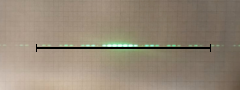
\includegraphics[width=\textwidth,page=1]{figuras/medidas/B4.pdf}}
  \begin{picture}(\wd\tempbox,\ht\tempbox)
    \put(0,0){\usebox{\tempbox}}
    \put(0,0){\includegraphics[width=\textwidth,page=2]{figuras/medidas/B4.pdf}}
    \put(.47\wd\tempbox,.37\ht\tempbox){$4~\Delta y$}
    \put(.48\wd\tempbox,.54\ht\tempbox){$5\Lambda$}
  \end{picture}
\endgroup


        \caption{B4}
        \label{fig:B4}
    \end{subfigure}
    \qquad
    \begin{subfigure}[t]{.6\textwidth}
        \centering
        \begingroup
  \sbox{\tempbox}{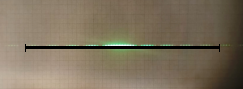
\includegraphics[width=\textwidth,page=1]{figuras/medidas/B5.pdf}}
  \begin{picture}(\wd\tempbox,\ht\tempbox)
    \put(0,0){\usebox{\tempbox}}
    \put(0,0){\includegraphics[width=\textwidth,page=2]{figuras/medidas/B5.pdf}}
    \put(.48\wd\tempbox,.37\ht\tempbox){$5~\Delta y$}
    \put(.46\wd\tempbox,.525\ht\tempbox){$11~\Lambda$}
  \end{picture}
\endgroup


        \caption{B5}
        \label{fig:B5}
    \end{subfigure}
    \qquad
    \begin{subfigure}[t]{.6\textwidth}
        \centering
        \begingroup
  \sbox{\tempbox}{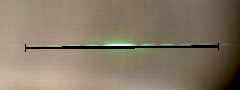
\includegraphics[width=\textwidth,page=1]{figuras/medidas/B6.pdf}}
  \begin{picture}(\wd\tempbox,\ht\tempbox)
    \put(0,0){\usebox{\tempbox}}
    \put(0,0){\includegraphics[width=\textwidth,page=2]{figuras/medidas/B6.pdf}}
    \put(.47\wd\tempbox,.38\ht\tempbox){$5~\Delta y$}
    \put(.595\wd\tempbox,.54\ht\tempbox){$6\Lambda$}
  \end{picture}
\endgroup


        \caption{B6}
        \label{fig:B6}
    \end{subfigure}

    \caption{Fotos dos padrões de difração das fendas B}
    \label{fig:B}
\end{figure}

\subsection{Fendas A}
\DTLloaddb{medidasA}{dados/A.csv}

\begin{table}[H]
	\centering
	\sisetup{
		table-figures-uncertainty = 1,
		zero-decimal-to-integer=false
	}
	\begin{tabular}{ccccccccc}
		\toprule\toprule
            {\bfseries Fenda} & {Número de fendas}
				& {\bfseries $n_y$}
				& {\bfseries $n_y \Delta y$ [\si{\milli\meter}]}
				& {\bfseries $\Delta y$ [\si{\milli\meter}]}
				& {\bfseries $n_\Lambda$}
				& {\bfseries $n_\Lambda \Lambda$ [\si{\milli\meter}]}
				& {\bfseries $\Lambda$ [\si{\milli\meter}]}
				& {\bfseries $\delta y$ [\si{\milli\meter}]}

		\DTLforeach*{medidasA}{\fenda=id,\nDy=nDy,\yr=yr,\n=n,\Dy=Dy,\Dyr=Dyr,\mL=mL,\m=m,\L=L,\Lr=Lr,\b=b,\br=br,\h=h,\hr=hr,\dy=dy,\dyr=dyr,\fendas=N}{
			\DTLiffirstrow{\\\midrule}{\\}
			\fenda & \fendas
				& $\num{\n}$
				& $\num{\nDy(\yr)}$
				& $\num{\Dy(\Dyr)}$
				& \ifdefempty{\m}{---}{$\num{\m}$}
				& \ifdefempty{\m}{---}{$\num{\mL(\yr)}$}
				& \ifdefempty{\m}{---}{$\num{\L(\Lr)}$}
				& \ifdefempty{\dy}{---}{$\num{\dy(\dyr)}$}
		}
        \\\bottomrule\bottomrule
	\end{tabular}

	\caption{Dados obtidos para os padrões de difração das fendas da linha A}
	\label{tab:fend_a}
\end{table}
\begin{figure}[H]
    \centering

    \begin{subfigure}[t]{.45\textwidth}
        \centering
        \begingroup
  \sbox{\tempbox}{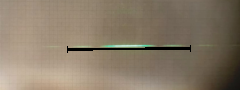
\includegraphics[width=\textwidth,page=1]{figuras/medidas/A1.pdf}}
  \begin{picture}(\wd\tempbox,\ht\tempbox)
    \put(0,0){\usebox{\tempbox}}
    \put(.48\wd\tempbox,.33\ht\tempbox){$2~\Delta y$}
  \end{picture}
\endgroup


        \caption{A1}
        \label{fig:A1}
    \end{subfigure}
    \qquad
    \begin{subfigure}[t]{.45\textwidth}
        \centering
        \begingroup
  \sbox{\tempbox}{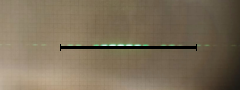
\includegraphics[width=\textwidth,page=1]{figuras/medidas/A2.pdf}}
  \begin{picture}(\wd\tempbox,\ht\tempbox)
    \put(0,0){\usebox{\tempbox}}
    \put(0,0){\includegraphics[width=\textwidth,page=2]{figuras/medidas/A2.pdf}}
    \put(.50\wd\tempbox,.35\ht\tempbox){$2~\Delta y$}
    \put(.485\wd\tempbox,.54\ht\tempbox){$6\Lambda$}
  \end{picture}
\endgroup


        \caption{A2}
        \label{fig:A2}
    \end{subfigure}
    \qquad
    \begin{subfigure}[t]{.45\textwidth}
        \centering
        \begingroup
  \sbox{\tempbox}{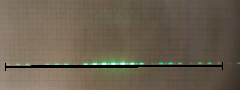
\includegraphics[width=\textwidth,page=1]{figuras/medidas/A3.pdf}}
  \begin{picture}(\wd\tempbox,\ht\tempbox)
    \put(0,0){\usebox{\tempbox}}
    \put(0,0){\includegraphics[width=\textwidth,page=2]{figuras/medidas/A3.pdf}}
    \put(.46\wd\tempbox,.15\ht\tempbox){$3~\Delta y$}
    \put(.44\wd\tempbox,.33\ht\tempbox){$2\delta y$}
  \end{picture}
\endgroup


        \caption{A3}
        \label{fig:A3}
    \end{subfigure}
    \qquad
    \begin{subfigure}[t]{.45\textwidth}
        \centering
        \begingroup
  \sbox{\tempbox}{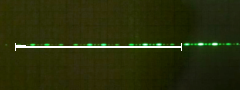
\includegraphics[width=\textwidth,page=1]{figuras/medidas/A4.pdf}}
  \begin{picture}(\wd\tempbox,\ht\tempbox)
    \put(0,0){\usebox{\tempbox}}
    \put(0,0){\includegraphics[width=\textwidth,page=2]{figuras/medidas/A4.pdf}}
    \put(.37\wd\tempbox,.35\ht\tempbox){\color{white}$1.5~\Delta y$}
    \put(.745\wd\tempbox,.56\ht\tempbox){\color{white}$2\delta y$}
  \end{picture}
\endgroup


        \caption{A4}
        \label{fig:A4}
    \end{subfigure}
    \qquad
    \begin{subfigure}[t]{.45\textwidth}
        \centering
        \begingroup
  \sbox{\tempbox}{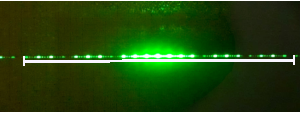
\includegraphics[width=\textwidth,page=1]{figuras/medidas/A5.pdf}}
  \begin{picture}(\wd\tempbox,\ht\tempbox)
    \put(0,0){\usebox{\tempbox}}
    \put(0,0){\includegraphics[width=\textwidth,page=2]{figuras/medidas/A5.pdf}}
    \put(.30\wd\tempbox,.33\ht\tempbox){\color{white}$3~\Delta y$}
    \put(.88\wd\tempbox,.54\ht\tempbox){\color{white}$2\delta y$}
  \end{picture}
\endgroup


        \caption{A5}
        \label{fig:A5}
    \end{subfigure}
    \qquad
    \begin{subfigure}[t]{.45\textwidth}
        \centering
        \begingroup
  \sbox{\tempbox}{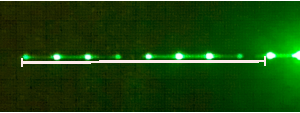
\includegraphics[width=\textwidth,page=1]{figuras/medidas/A6.pdf}}
  \begin{picture}(\wd\tempbox,\ht\tempbox)
    \put(0,0){\usebox{\tempbox}}
    \put(0,0){\includegraphics[width=\textwidth,page=2]{figuras/medidas/A6.pdf}}
    \put(.42\wd\tempbox,.32\ht\tempbox){\color{white}$1~\Delta y$}
    \put(.46\wd\tempbox,.56\ht\tempbox){\color{white}$2\delta y$}
  \end{picture}
\endgroup


        \caption{A6}
        \label{fig:A6}
    \end{subfigure}

    \caption{Fotos dos padrões de difração das fendas A}
    \label{fig:A}
\end{figure}
\begin{table}[H]
	\centering
	\sisetup{
		table-figures-uncertainty = 1,
		zero-decimal-to-integer = false
	}
	\begin{tabular}{cccccc}
		\toprule\toprule
            \multirow{2}*{\bfseries Fenda} & \multirow{2}*{Número de fendas}
				& \multicolumn{2}{c}{\bfseries $b$ [\si{\micro\meter}]}
				& \multicolumn{2}{c}{\bfseries $h$ [\si{\micro\meter}]}
			\\ & & Calculado & Microscópio & Calculado & Microscópio

		\DTLforeach*{medidasA}{\fenda=id,\nDy=nDy,\yr=yr,\n=n,\Dy=Dy,\Dyr=Dyr,\mL=mL,\m=m,\L=L,\Lr=Lr,\b=b,\br=br,\h=h,\hr=hr,\dy=dy,\dyr=dyr,\fendas=N}{
			\DTLiffirstrow{\\\midrule}{\\}
			\fenda & \fendas
				& $\num{\b(\br)}$
				& $\num{24.0(9)}$
				& \ifdefempty{\h}{---}{$\num{\h(\hr)}$}
				& \ifdefempty{\h}{---}{$\num{100.0(9)}$}
		}
        \\\bottomrule\bottomrule
	\end{tabular}

	\caption{Dimensões encontradas para cada fenda da linha A}
	\label{tab:fend_a2}
\end{table}
%% Creator: Matplotlib, PGF backend
%%
%% To include the figure in your LaTeX document, write
%%   \input{<filename>.pgf}
%%
%% Make sure the required packages are loaded in your preamble
%%   \usepackage{pgf}
%%
%% Figures using additional raster images can only be included by \input if
%% they are in the same directory as the main LaTeX file. For loading figures
%% from other directories you can use the `import` package
%%   \usepackage{import}
%% and then include the figures with
%%   \import{<path to file>}{<filename>.pgf}
%%
%% Matplotlib used the following preamble
%%   \usepackage[utf8]{inputenc}
%%   \usepackage[T1]{fontenc}
%%   \usepackage[portuguese]{babel}
%%   \usepackage{siunitx}
%%   \usepackage{gensymb}
%%   \usepackage{fontspec}
%%   \setmainfont{DejaVuSerif.ttf}[Path=/home/marmis/.virtualenvs/default/lib/python3.7/site-packages/matplotlib/mpl-data/fonts/ttf/]
%%   \setsansfont{arial.ttf}[Path=/usr/share/fonts/TTF/]
%%   \setmonofont{DejaVuSansMono.ttf}[Path=/home/marmis/.virtualenvs/default/lib/python3.7/site-packages/matplotlib/mpl-data/fonts/ttf/]
%%
\begingroup%
\makeatletter%
\begin{pgfpicture}%
\pgfpathrectangle{\pgfpointorigin}{\pgfqpoint{5.000000in}{3.000000in}}%
\pgfusepath{use as bounding box, clip}%
\begin{pgfscope}%
\pgfsetbuttcap%
\pgfsetmiterjoin%
\definecolor{currentfill}{rgb}{1.000000,1.000000,1.000000}%
\pgfsetfillcolor{currentfill}%
\pgfsetlinewidth{0.000000pt}%
\definecolor{currentstroke}{rgb}{1.000000,1.000000,1.000000}%
\pgfsetstrokecolor{currentstroke}%
\pgfsetdash{}{0pt}%
\pgfpathmoveto{\pgfqpoint{0.000000in}{0.000000in}}%
\pgfpathlineto{\pgfqpoint{5.000000in}{0.000000in}}%
\pgfpathlineto{\pgfqpoint{5.000000in}{3.000000in}}%
\pgfpathlineto{\pgfqpoint{0.000000in}{3.000000in}}%
\pgfpathclose%
\pgfusepath{fill}%
\end{pgfscope}%
\begin{pgfscope}%
\pgfsetbuttcap%
\pgfsetmiterjoin%
\definecolor{currentfill}{rgb}{0.917647,0.917647,0.949020}%
\pgfsetfillcolor{currentfill}%
\pgfsetlinewidth{0.000000pt}%
\definecolor{currentstroke}{rgb}{0.000000,0.000000,0.000000}%
\pgfsetstrokecolor{currentstroke}%
\pgfsetstrokeopacity{0.000000}%
\pgfsetdash{}{0pt}%
\pgfpathmoveto{\pgfqpoint{0.837708in}{0.562153in}}%
\pgfpathlineto{\pgfqpoint{4.808000in}{0.562153in}}%
\pgfpathlineto{\pgfqpoint{4.808000in}{2.666026in}}%
\pgfpathlineto{\pgfqpoint{0.837708in}{2.666026in}}%
\pgfpathclose%
\pgfusepath{fill}%
\end{pgfscope}%
\begin{pgfscope}%
\pgfpathrectangle{\pgfqpoint{0.837708in}{0.562153in}}{\pgfqpoint{3.970292in}{2.103873in}}%
\pgfusepath{clip}%
\pgfsetroundcap%
\pgfsetroundjoin%
\pgfsetlinewidth{0.803000pt}%
\definecolor{currentstroke}{rgb}{1.000000,1.000000,1.000000}%
\pgfsetstrokecolor{currentstroke}%
\pgfsetdash{}{0pt}%
\pgfpathmoveto{\pgfqpoint{4.724680in}{0.562153in}}%
\pgfpathlineto{\pgfqpoint{4.724680in}{2.666026in}}%
\pgfusepath{stroke}%
\end{pgfscope}%
\begin{pgfscope}%
\pgfsetbuttcap%
\pgfsetroundjoin%
\definecolor{currentfill}{rgb}{0.411765,0.411765,0.411765}%
\pgfsetfillcolor{currentfill}%
\pgfsetlinewidth{1.003750pt}%
\definecolor{currentstroke}{rgb}{0.411765,0.411765,0.411765}%
\pgfsetstrokecolor{currentstroke}%
\pgfsetdash{}{0pt}%
\pgfsys@defobject{currentmarker}{\pgfqpoint{0.000000in}{-0.066667in}}{\pgfqpoint{0.000000in}{0.000000in}}{%
\pgfpathmoveto{\pgfqpoint{0.000000in}{0.000000in}}%
\pgfpathlineto{\pgfqpoint{0.000000in}{-0.066667in}}%
\pgfusepath{stroke,fill}%
}%
\begin{pgfscope}%
\pgfsys@transformshift{4.724680in}{0.562153in}%
\pgfsys@useobject{currentmarker}{}%
\end{pgfscope}%
\end{pgfscope}%
\begin{pgfscope}%
\definecolor{textcolor}{rgb}{0.411765,0.411765,0.411765}%
\pgfsetstrokecolor{textcolor}%
\pgfsetfillcolor{textcolor}%
\pgftext[x=4.724680in,y=0.446875in,,top]{\color{textcolor}\rmfamily\fontsize{8.800000}{10.560000}\selectfont \(\displaystyle 10^{1}\)}%
\end{pgfscope}%
\begin{pgfscope}%
\pgfsetbuttcap%
\pgfsetroundjoin%
\definecolor{currentfill}{rgb}{0.411765,0.411765,0.411765}%
\pgfsetfillcolor{currentfill}%
\pgfsetlinewidth{0.803000pt}%
\definecolor{currentstroke}{rgb}{0.411765,0.411765,0.411765}%
\pgfsetstrokecolor{currentstroke}%
\pgfsetdash{}{0pt}%
\pgfsys@defobject{currentmarker}{\pgfqpoint{0.000000in}{-0.044444in}}{\pgfqpoint{0.000000in}{0.000000in}}{%
\pgfpathmoveto{\pgfqpoint{0.000000in}{0.000000in}}%
\pgfpathlineto{\pgfqpoint{0.000000in}{-0.044444in}}%
\pgfusepath{stroke,fill}%
}%
\begin{pgfscope}%
\pgfsys@transformshift{1.311876in}{0.562153in}%
\pgfsys@useobject{currentmarker}{}%
\end{pgfscope}%
\end{pgfscope}%
\begin{pgfscope}%
\definecolor{textcolor}{rgb}{0.411765,0.411765,0.411765}%
\pgfsetstrokecolor{textcolor}%
\pgfsetfillcolor{textcolor}%
\pgftext[x=1.311876in,y=0.470486in,,top]{\color{textcolor}\rmfamily\fontsize{8.800000}{10.560000}\selectfont \(\displaystyle 2\times10^{0}\)}%
\end{pgfscope}%
\begin{pgfscope}%
\pgfsetbuttcap%
\pgfsetroundjoin%
\definecolor{currentfill}{rgb}{0.411765,0.411765,0.411765}%
\pgfsetfillcolor{currentfill}%
\pgfsetlinewidth{0.803000pt}%
\definecolor{currentstroke}{rgb}{0.411765,0.411765,0.411765}%
\pgfsetstrokecolor{currentstroke}%
\pgfsetdash{}{0pt}%
\pgfsys@defobject{currentmarker}{\pgfqpoint{0.000000in}{-0.044444in}}{\pgfqpoint{0.000000in}{0.000000in}}{%
\pgfpathmoveto{\pgfqpoint{0.000000in}{0.000000in}}%
\pgfpathlineto{\pgfqpoint{0.000000in}{-0.044444in}}%
\pgfusepath{stroke,fill}%
}%
\begin{pgfscope}%
\pgfsys@transformshift{2.171663in}{0.562153in}%
\pgfsys@useobject{currentmarker}{}%
\end{pgfscope}%
\end{pgfscope}%
\begin{pgfscope}%
\definecolor{textcolor}{rgb}{0.411765,0.411765,0.411765}%
\pgfsetstrokecolor{textcolor}%
\pgfsetfillcolor{textcolor}%
\pgftext[x=2.171663in,y=0.470486in,,top]{\color{textcolor}\rmfamily\fontsize{8.800000}{10.560000}\selectfont \(\displaystyle 3\times10^{0}\)}%
\end{pgfscope}%
\begin{pgfscope}%
\pgfsetbuttcap%
\pgfsetroundjoin%
\definecolor{currentfill}{rgb}{0.411765,0.411765,0.411765}%
\pgfsetfillcolor{currentfill}%
\pgfsetlinewidth{0.803000pt}%
\definecolor{currentstroke}{rgb}{0.411765,0.411765,0.411765}%
\pgfsetstrokecolor{currentstroke}%
\pgfsetdash{}{0pt}%
\pgfsys@defobject{currentmarker}{\pgfqpoint{0.000000in}{-0.044444in}}{\pgfqpoint{0.000000in}{0.000000in}}{%
\pgfpathmoveto{\pgfqpoint{0.000000in}{0.000000in}}%
\pgfpathlineto{\pgfqpoint{0.000000in}{-0.044444in}}%
\pgfusepath{stroke,fill}%
}%
\begin{pgfscope}%
\pgfsys@transformshift{2.781691in}{0.562153in}%
\pgfsys@useobject{currentmarker}{}%
\end{pgfscope}%
\end{pgfscope}%
\begin{pgfscope}%
\definecolor{textcolor}{rgb}{0.411765,0.411765,0.411765}%
\pgfsetstrokecolor{textcolor}%
\pgfsetfillcolor{textcolor}%
\pgftext[x=2.781691in,y=0.470486in,,top]{\color{textcolor}\rmfamily\fontsize{8.800000}{10.560000}\selectfont \(\displaystyle 4\times10^{0}\)}%
\end{pgfscope}%
\begin{pgfscope}%
\pgfsetbuttcap%
\pgfsetroundjoin%
\definecolor{currentfill}{rgb}{0.411765,0.411765,0.411765}%
\pgfsetfillcolor{currentfill}%
\pgfsetlinewidth{0.803000pt}%
\definecolor{currentstroke}{rgb}{0.411765,0.411765,0.411765}%
\pgfsetstrokecolor{currentstroke}%
\pgfsetdash{}{0pt}%
\pgfsys@defobject{currentmarker}{\pgfqpoint{0.000000in}{-0.044444in}}{\pgfqpoint{0.000000in}{0.000000in}}{%
\pgfpathmoveto{\pgfqpoint{0.000000in}{0.000000in}}%
\pgfpathlineto{\pgfqpoint{0.000000in}{-0.044444in}}%
\pgfusepath{stroke,fill}%
}%
\begin{pgfscope}%
\pgfsys@transformshift{3.254865in}{0.562153in}%
\pgfsys@useobject{currentmarker}{}%
\end{pgfscope}%
\end{pgfscope}%
\begin{pgfscope}%
\pgfsetbuttcap%
\pgfsetroundjoin%
\definecolor{currentfill}{rgb}{0.411765,0.411765,0.411765}%
\pgfsetfillcolor{currentfill}%
\pgfsetlinewidth{0.803000pt}%
\definecolor{currentstroke}{rgb}{0.411765,0.411765,0.411765}%
\pgfsetstrokecolor{currentstroke}%
\pgfsetdash{}{0pt}%
\pgfsys@defobject{currentmarker}{\pgfqpoint{0.000000in}{-0.044444in}}{\pgfqpoint{0.000000in}{0.000000in}}{%
\pgfpathmoveto{\pgfqpoint{0.000000in}{0.000000in}}%
\pgfpathlineto{\pgfqpoint{0.000000in}{-0.044444in}}%
\pgfusepath{stroke,fill}%
}%
\begin{pgfscope}%
\pgfsys@transformshift{3.641477in}{0.562153in}%
\pgfsys@useobject{currentmarker}{}%
\end{pgfscope}%
\end{pgfscope}%
\begin{pgfscope}%
\definecolor{textcolor}{rgb}{0.411765,0.411765,0.411765}%
\pgfsetstrokecolor{textcolor}%
\pgfsetfillcolor{textcolor}%
\pgftext[x=3.641477in,y=0.470486in,,top]{\color{textcolor}\rmfamily\fontsize{8.800000}{10.560000}\selectfont \(\displaystyle 6\times10^{0}\)}%
\end{pgfscope}%
\begin{pgfscope}%
\pgfsetbuttcap%
\pgfsetroundjoin%
\definecolor{currentfill}{rgb}{0.411765,0.411765,0.411765}%
\pgfsetfillcolor{currentfill}%
\pgfsetlinewidth{0.803000pt}%
\definecolor{currentstroke}{rgb}{0.411765,0.411765,0.411765}%
\pgfsetstrokecolor{currentstroke}%
\pgfsetdash{}{0pt}%
\pgfsys@defobject{currentmarker}{\pgfqpoint{0.000000in}{-0.044444in}}{\pgfqpoint{0.000000in}{0.000000in}}{%
\pgfpathmoveto{\pgfqpoint{0.000000in}{0.000000in}}%
\pgfpathlineto{\pgfqpoint{0.000000in}{-0.044444in}}%
\pgfusepath{stroke,fill}%
}%
\begin{pgfscope}%
\pgfsys@transformshift{3.968353in}{0.562153in}%
\pgfsys@useobject{currentmarker}{}%
\end{pgfscope}%
\end{pgfscope}%
\begin{pgfscope}%
\pgfsetbuttcap%
\pgfsetroundjoin%
\definecolor{currentfill}{rgb}{0.411765,0.411765,0.411765}%
\pgfsetfillcolor{currentfill}%
\pgfsetlinewidth{0.803000pt}%
\definecolor{currentstroke}{rgb}{0.411765,0.411765,0.411765}%
\pgfsetstrokecolor{currentstroke}%
\pgfsetdash{}{0pt}%
\pgfsys@defobject{currentmarker}{\pgfqpoint{0.000000in}{-0.044444in}}{\pgfqpoint{0.000000in}{0.000000in}}{%
\pgfpathmoveto{\pgfqpoint{0.000000in}{0.000000in}}%
\pgfpathlineto{\pgfqpoint{0.000000in}{-0.044444in}}%
\pgfusepath{stroke,fill}%
}%
\begin{pgfscope}%
\pgfsys@transformshift{4.251505in}{0.562153in}%
\pgfsys@useobject{currentmarker}{}%
\end{pgfscope}%
\end{pgfscope}%
\begin{pgfscope}%
\pgfsetbuttcap%
\pgfsetroundjoin%
\definecolor{currentfill}{rgb}{0.411765,0.411765,0.411765}%
\pgfsetfillcolor{currentfill}%
\pgfsetlinewidth{0.803000pt}%
\definecolor{currentstroke}{rgb}{0.411765,0.411765,0.411765}%
\pgfsetstrokecolor{currentstroke}%
\pgfsetdash{}{0pt}%
\pgfsys@defobject{currentmarker}{\pgfqpoint{0.000000in}{-0.044444in}}{\pgfqpoint{0.000000in}{0.000000in}}{%
\pgfpathmoveto{\pgfqpoint{0.000000in}{0.000000in}}%
\pgfpathlineto{\pgfqpoint{0.000000in}{-0.044444in}}%
\pgfusepath{stroke,fill}%
}%
\begin{pgfscope}%
\pgfsys@transformshift{4.501264in}{0.562153in}%
\pgfsys@useobject{currentmarker}{}%
\end{pgfscope}%
\end{pgfscope}%
\begin{pgfscope}%
\definecolor{textcolor}{rgb}{0.000000,0.000000,0.000000}%
\pgfsetstrokecolor{textcolor}%
\pgfsetfillcolor{textcolor}%
\pgftext[x=2.822854in,y=0.273036in,,top]{\color{textcolor}\rmfamily\fontsize{9.600000}{11.520000}\selectfont \(\displaystyle N\)}%
\end{pgfscope}%
\begin{pgfscope}%
\pgfpathrectangle{\pgfqpoint{0.837708in}{0.562153in}}{\pgfqpoint{3.970292in}{2.103873in}}%
\pgfusepath{clip}%
\pgfsetroundcap%
\pgfsetroundjoin%
\pgfsetlinewidth{0.803000pt}%
\definecolor{currentstroke}{rgb}{1.000000,1.000000,1.000000}%
\pgfsetstrokecolor{currentstroke}%
\pgfsetdash{}{0pt}%
\pgfpathmoveto{\pgfqpoint{0.837708in}{0.724945in}}%
\pgfpathlineto{\pgfqpoint{4.808000in}{0.724945in}}%
\pgfusepath{stroke}%
\end{pgfscope}%
\begin{pgfscope}%
\pgfsetbuttcap%
\pgfsetroundjoin%
\definecolor{currentfill}{rgb}{0.411765,0.411765,0.411765}%
\pgfsetfillcolor{currentfill}%
\pgfsetlinewidth{1.003750pt}%
\definecolor{currentstroke}{rgb}{0.411765,0.411765,0.411765}%
\pgfsetstrokecolor{currentstroke}%
\pgfsetdash{}{0pt}%
\pgfsys@defobject{currentmarker}{\pgfqpoint{-0.066667in}{0.000000in}}{\pgfqpoint{0.000000in}{0.000000in}}{%
\pgfpathmoveto{\pgfqpoint{0.000000in}{0.000000in}}%
\pgfpathlineto{\pgfqpoint{-0.066667in}{0.000000in}}%
\pgfusepath{stroke,fill}%
}%
\begin{pgfscope}%
\pgfsys@transformshift{0.837708in}{0.724945in}%
\pgfsys@useobject{currentmarker}{}%
\end{pgfscope}%
\end{pgfscope}%
\begin{pgfscope}%
\definecolor{textcolor}{rgb}{0.411765,0.411765,0.411765}%
\pgfsetstrokecolor{textcolor}%
\pgfsetfillcolor{textcolor}%
\pgftext[x=0.536090in,y=0.678515in,left,base]{\color{textcolor}\rmfamily\fontsize{8.800000}{10.560000}\selectfont \(\displaystyle 10^{0}\)}%
\end{pgfscope}%
\begin{pgfscope}%
\pgfsetbuttcap%
\pgfsetroundjoin%
\definecolor{currentfill}{rgb}{0.411765,0.411765,0.411765}%
\pgfsetfillcolor{currentfill}%
\pgfsetlinewidth{0.803000pt}%
\definecolor{currentstroke}{rgb}{0.411765,0.411765,0.411765}%
\pgfsetstrokecolor{currentstroke}%
\pgfsetdash{}{0pt}%
\pgfsys@defobject{currentmarker}{\pgfqpoint{-0.044444in}{0.000000in}}{\pgfqpoint{0.000000in}{0.000000in}}{%
\pgfpathmoveto{\pgfqpoint{0.000000in}{0.000000in}}%
\pgfpathlineto{\pgfqpoint{-0.044444in}{0.000000in}}%
\pgfusepath{stroke,fill}%
}%
\begin{pgfscope}%
\pgfsys@transformshift{0.837708in}{0.619820in}%
\pgfsys@useobject{currentmarker}{}%
\end{pgfscope}%
\end{pgfscope}%
\begin{pgfscope}%
\pgfsetbuttcap%
\pgfsetroundjoin%
\definecolor{currentfill}{rgb}{0.411765,0.411765,0.411765}%
\pgfsetfillcolor{currentfill}%
\pgfsetlinewidth{0.803000pt}%
\definecolor{currentstroke}{rgb}{0.411765,0.411765,0.411765}%
\pgfsetstrokecolor{currentstroke}%
\pgfsetdash{}{0pt}%
\pgfsys@defobject{currentmarker}{\pgfqpoint{-0.044444in}{0.000000in}}{\pgfqpoint{0.000000in}{0.000000in}}{%
\pgfpathmoveto{\pgfqpoint{0.000000in}{0.000000in}}%
\pgfpathlineto{\pgfqpoint{-0.044444in}{0.000000in}}%
\pgfusepath{stroke,fill}%
}%
\begin{pgfscope}%
\pgfsys@transformshift{0.837708in}{1.416544in}%
\pgfsys@useobject{currentmarker}{}%
\end{pgfscope}%
\end{pgfscope}%
\begin{pgfscope}%
\definecolor{textcolor}{rgb}{0.411765,0.411765,0.411765}%
\pgfsetstrokecolor{textcolor}%
\pgfsetfillcolor{textcolor}%
\pgftext[x=0.338444in,y=1.366594in,left,base]{\color{textcolor}\rmfamily\fontsize{8.800000}{10.560000}\selectfont \(\displaystyle 2\times10^{0}\)}%
\end{pgfscope}%
\begin{pgfscope}%
\pgfsetbuttcap%
\pgfsetroundjoin%
\definecolor{currentfill}{rgb}{0.411765,0.411765,0.411765}%
\pgfsetfillcolor{currentfill}%
\pgfsetlinewidth{0.803000pt}%
\definecolor{currentstroke}{rgb}{0.411765,0.411765,0.411765}%
\pgfsetstrokecolor{currentstroke}%
\pgfsetdash{}{0pt}%
\pgfsys@defobject{currentmarker}{\pgfqpoint{-0.044444in}{0.000000in}}{\pgfqpoint{0.000000in}{0.000000in}}{%
\pgfpathmoveto{\pgfqpoint{0.000000in}{0.000000in}}%
\pgfpathlineto{\pgfqpoint{-0.044444in}{0.000000in}}%
\pgfusepath{stroke,fill}%
}%
\begin{pgfscope}%
\pgfsys@transformshift{0.837708in}{1.821103in}%
\pgfsys@useobject{currentmarker}{}%
\end{pgfscope}%
\end{pgfscope}%
\begin{pgfscope}%
\definecolor{textcolor}{rgb}{0.411765,0.411765,0.411765}%
\pgfsetstrokecolor{textcolor}%
\pgfsetfillcolor{textcolor}%
\pgftext[x=0.338444in,y=1.771153in,left,base]{\color{textcolor}\rmfamily\fontsize{8.800000}{10.560000}\selectfont \(\displaystyle 3\times10^{0}\)}%
\end{pgfscope}%
\begin{pgfscope}%
\pgfsetbuttcap%
\pgfsetroundjoin%
\definecolor{currentfill}{rgb}{0.411765,0.411765,0.411765}%
\pgfsetfillcolor{currentfill}%
\pgfsetlinewidth{0.803000pt}%
\definecolor{currentstroke}{rgb}{0.411765,0.411765,0.411765}%
\pgfsetstrokecolor{currentstroke}%
\pgfsetdash{}{0pt}%
\pgfsys@defobject{currentmarker}{\pgfqpoint{-0.044444in}{0.000000in}}{\pgfqpoint{0.000000in}{0.000000in}}{%
\pgfpathmoveto{\pgfqpoint{0.000000in}{0.000000in}}%
\pgfpathlineto{\pgfqpoint{-0.044444in}{0.000000in}}%
\pgfusepath{stroke,fill}%
}%
\begin{pgfscope}%
\pgfsys@transformshift{0.837708in}{2.108143in}%
\pgfsys@useobject{currentmarker}{}%
\end{pgfscope}%
\end{pgfscope}%
\begin{pgfscope}%
\definecolor{textcolor}{rgb}{0.411765,0.411765,0.411765}%
\pgfsetstrokecolor{textcolor}%
\pgfsetfillcolor{textcolor}%
\pgftext[x=0.338444in,y=2.058193in,left,base]{\color{textcolor}\rmfamily\fontsize{8.800000}{10.560000}\selectfont \(\displaystyle 4\times10^{0}\)}%
\end{pgfscope}%
\begin{pgfscope}%
\pgfsetbuttcap%
\pgfsetroundjoin%
\definecolor{currentfill}{rgb}{0.411765,0.411765,0.411765}%
\pgfsetfillcolor{currentfill}%
\pgfsetlinewidth{0.803000pt}%
\definecolor{currentstroke}{rgb}{0.411765,0.411765,0.411765}%
\pgfsetstrokecolor{currentstroke}%
\pgfsetdash{}{0pt}%
\pgfsys@defobject{currentmarker}{\pgfqpoint{-0.044444in}{0.000000in}}{\pgfqpoint{0.000000in}{0.000000in}}{%
\pgfpathmoveto{\pgfqpoint{0.000000in}{0.000000in}}%
\pgfpathlineto{\pgfqpoint{-0.044444in}{0.000000in}}%
\pgfusepath{stroke,fill}%
}%
\begin{pgfscope}%
\pgfsys@transformshift{0.837708in}{2.330788in}%
\pgfsys@useobject{currentmarker}{}%
\end{pgfscope}%
\end{pgfscope}%
\begin{pgfscope}%
\pgfsetbuttcap%
\pgfsetroundjoin%
\definecolor{currentfill}{rgb}{0.411765,0.411765,0.411765}%
\pgfsetfillcolor{currentfill}%
\pgfsetlinewidth{0.803000pt}%
\definecolor{currentstroke}{rgb}{0.411765,0.411765,0.411765}%
\pgfsetstrokecolor{currentstroke}%
\pgfsetdash{}{0pt}%
\pgfsys@defobject{currentmarker}{\pgfqpoint{-0.044444in}{0.000000in}}{\pgfqpoint{0.000000in}{0.000000in}}{%
\pgfpathmoveto{\pgfqpoint{0.000000in}{0.000000in}}%
\pgfpathlineto{\pgfqpoint{-0.044444in}{0.000000in}}%
\pgfusepath{stroke,fill}%
}%
\begin{pgfscope}%
\pgfsys@transformshift{0.837708in}{2.512702in}%
\pgfsys@useobject{currentmarker}{}%
\end{pgfscope}%
\end{pgfscope}%
\begin{pgfscope}%
\definecolor{textcolor}{rgb}{0.411765,0.411765,0.411765}%
\pgfsetstrokecolor{textcolor}%
\pgfsetfillcolor{textcolor}%
\pgftext[x=0.338444in,y=2.462752in,left,base]{\color{textcolor}\rmfamily\fontsize{8.800000}{10.560000}\selectfont \(\displaystyle 6\times10^{0}\)}%
\end{pgfscope}%
\begin{pgfscope}%
\pgfsetbuttcap%
\pgfsetroundjoin%
\definecolor{currentfill}{rgb}{0.411765,0.411765,0.411765}%
\pgfsetfillcolor{currentfill}%
\pgfsetlinewidth{0.803000pt}%
\definecolor{currentstroke}{rgb}{0.411765,0.411765,0.411765}%
\pgfsetstrokecolor{currentstroke}%
\pgfsetdash{}{0pt}%
\pgfsys@defobject{currentmarker}{\pgfqpoint{-0.044444in}{0.000000in}}{\pgfqpoint{0.000000in}{0.000000in}}{%
\pgfpathmoveto{\pgfqpoint{0.000000in}{0.000000in}}%
\pgfpathlineto{\pgfqpoint{-0.044444in}{0.000000in}}%
\pgfusepath{stroke,fill}%
}%
\begin{pgfscope}%
\pgfsys@transformshift{0.837708in}{2.666509in}%
\pgfsys@useobject{currentmarker}{}%
\end{pgfscope}%
\end{pgfscope}%
\begin{pgfscope}%
\definecolor{textcolor}{rgb}{0.000000,0.000000,0.000000}%
\pgfsetstrokecolor{textcolor}%
\pgfsetfillcolor{textcolor}%
\pgftext[x=0.282889in,y=1.614090in,,bottom,rotate=90.000000]{\color{textcolor}\rmfamily\fontsize{9.600000}{11.520000}\selectfont \(\displaystyle \delta y\) \(\displaystyle \left[\si{\milli\meter}\right]\)}%
\end{pgfscope}%
\begin{pgfscope}%
\pgfpathrectangle{\pgfqpoint{0.837708in}{0.562153in}}{\pgfqpoint{3.970292in}{2.103873in}}%
\pgfusepath{clip}%
\pgfsetbuttcap%
\pgfsetroundjoin%
\definecolor{currentfill}{rgb}{0.100000,0.100000,0.100000}%
\pgfsetfillcolor{currentfill}%
\pgfsetfillopacity{0.150000}%
\pgfsetlinewidth{0.803000pt}%
\definecolor{currentstroke}{rgb}{0.100000,0.100000,0.100000}%
\pgfsetstrokecolor{currentstroke}%
\pgfsetstrokeopacity{0.150000}%
\pgfsetdash{}{0pt}%
\pgfpathmoveto{\pgfqpoint{0.837708in}{2.570395in}}%
\pgfpathlineto{\pgfqpoint{0.837708in}{2.528284in}}%
\pgfpathlineto{\pgfqpoint{0.895556in}{2.501152in}}%
\pgfpathlineto{\pgfqpoint{0.951868in}{2.474741in}}%
\pgfpathlineto{\pgfqpoint{1.006722in}{2.449013in}}%
\pgfpathlineto{\pgfqpoint{1.060194in}{2.423934in}}%
\pgfpathlineto{\pgfqpoint{1.112350in}{2.399471in}}%
\pgfpathlineto{\pgfqpoint{1.163254in}{2.375594in}}%
\pgfpathlineto{\pgfqpoint{1.212964in}{2.352277in}}%
\pgfpathlineto{\pgfqpoint{1.261536in}{2.329494in}}%
\pgfpathlineto{\pgfqpoint{1.309021in}{2.307219in}}%
\pgfpathlineto{\pgfqpoint{1.355465in}{2.285433in}}%
\pgfpathlineto{\pgfqpoint{1.400913in}{2.264112in}}%
\pgfpathlineto{\pgfqpoint{1.445408in}{2.243238in}}%
\pgfpathlineto{\pgfqpoint{1.488989in}{2.222792in}}%
\pgfpathlineto{\pgfqpoint{1.531692in}{2.202757in}}%
\pgfpathlineto{\pgfqpoint{1.573551in}{2.183117in}}%
\pgfpathlineto{\pgfqpoint{1.614601in}{2.163856in}}%
\pgfpathlineto{\pgfqpoint{1.654871in}{2.144960in}}%
\pgfpathlineto{\pgfqpoint{1.694390in}{2.126415in}}%
\pgfpathlineto{\pgfqpoint{1.733186in}{2.108208in}}%
\pgfpathlineto{\pgfqpoint{1.771285in}{2.090328in}}%
\pgfpathlineto{\pgfqpoint{1.808712in}{2.072762in}}%
\pgfpathlineto{\pgfqpoint{1.845490in}{2.055500in}}%
\pgfpathlineto{\pgfqpoint{1.881640in}{2.038532in}}%
\pgfpathlineto{\pgfqpoint{1.917185in}{2.021846in}}%
\pgfpathlineto{\pgfqpoint{1.952143in}{2.005435in}}%
\pgfpathlineto{\pgfqpoint{1.986535in}{1.989289in}}%
\pgfpathlineto{\pgfqpoint{2.020378in}{1.973400in}}%
\pgfpathlineto{\pgfqpoint{2.053689in}{1.957759in}}%
\pgfpathlineto{\pgfqpoint{2.086484in}{1.942360in}}%
\pgfpathlineto{\pgfqpoint{2.118781in}{1.927193in}}%
\pgfpathlineto{\pgfqpoint{2.150593in}{1.912254in}}%
\pgfpathlineto{\pgfqpoint{2.181934in}{1.897534in}}%
\pgfpathlineto{\pgfqpoint{2.212819in}{1.883027in}}%
\pgfpathlineto{\pgfqpoint{2.243261in}{1.868728in}}%
\pgfpathlineto{\pgfqpoint{2.273272in}{1.854630in}}%
\pgfpathlineto{\pgfqpoint{2.302864in}{1.840728in}}%
\pgfpathlineto{\pgfqpoint{2.332049in}{1.827016in}}%
\pgfpathlineto{\pgfqpoint{2.360837in}{1.813489in}}%
\pgfpathlineto{\pgfqpoint{2.389240in}{1.800143in}}%
\pgfpathlineto{\pgfqpoint{2.417268in}{1.786972in}}%
\pgfpathlineto{\pgfqpoint{2.444930in}{1.773971in}}%
\pgfpathlineto{\pgfqpoint{2.472235in}{1.761138in}}%
\pgfpathlineto{\pgfqpoint{2.499194in}{1.748466in}}%
\pgfpathlineto{\pgfqpoint{2.525814in}{1.735953in}}%
\pgfpathlineto{\pgfqpoint{2.552104in}{1.723594in}}%
\pgfpathlineto{\pgfqpoint{2.578072in}{1.711385in}}%
\pgfpathlineto{\pgfqpoint{2.603726in}{1.699323in}}%
\pgfpathlineto{\pgfqpoint{2.629073in}{1.687404in}}%
\pgfpathlineto{\pgfqpoint{2.654121in}{1.675625in}}%
\pgfpathlineto{\pgfqpoint{2.678876in}{1.663983in}}%
\pgfpathlineto{\pgfqpoint{2.703346in}{1.652474in}}%
\pgfpathlineto{\pgfqpoint{2.727537in}{1.641095in}}%
\pgfpathlineto{\pgfqpoint{2.751455in}{1.629844in}}%
\pgfpathlineto{\pgfqpoint{2.775106in}{1.618718in}}%
\pgfpathlineto{\pgfqpoint{2.798496in}{1.607713in}}%
\pgfpathlineto{\pgfqpoint{2.821630in}{1.596828in}}%
\pgfpathlineto{\pgfqpoint{2.844516in}{1.586059in}}%
\pgfpathlineto{\pgfqpoint{2.867157in}{1.575405in}}%
\pgfpathlineto{\pgfqpoint{2.889558in}{1.564862in}}%
\pgfpathlineto{\pgfqpoint{2.911726in}{1.554428in}}%
\pgfpathlineto{\pgfqpoint{2.933664in}{1.544102in}}%
\pgfpathlineto{\pgfqpoint{2.955377in}{1.533880in}}%
\pgfpathlineto{\pgfqpoint{2.976871in}{1.523762in}}%
\pgfpathlineto{\pgfqpoint{2.998149in}{1.513744in}}%
\pgfpathlineto{\pgfqpoint{3.019215in}{1.503824in}}%
\pgfpathlineto{\pgfqpoint{3.040074in}{1.494002in}}%
\pgfpathlineto{\pgfqpoint{3.060730in}{1.484274in}}%
\pgfpathlineto{\pgfqpoint{3.081187in}{1.474640in}}%
\pgfpathlineto{\pgfqpoint{3.101448in}{1.465097in}}%
\pgfpathlineto{\pgfqpoint{3.121517in}{1.455643in}}%
\pgfpathlineto{\pgfqpoint{3.141398in}{1.446277in}}%
\pgfpathlineto{\pgfqpoint{3.161095in}{1.436998in}}%
\pgfpathlineto{\pgfqpoint{3.180610in}{1.427803in}}%
\pgfpathlineto{\pgfqpoint{3.199948in}{1.418691in}}%
\pgfpathlineto{\pgfqpoint{3.219110in}{1.409661in}}%
\pgfpathlineto{\pgfqpoint{3.238101in}{1.400711in}}%
\pgfpathlineto{\pgfqpoint{3.256924in}{1.391840in}}%
\pgfpathlineto{\pgfqpoint{3.275581in}{1.383046in}}%
\pgfpathlineto{\pgfqpoint{3.294075in}{1.374328in}}%
\pgfpathlineto{\pgfqpoint{3.312409in}{1.365685in}}%
\pgfpathlineto{\pgfqpoint{3.330586in}{1.357115in}}%
\pgfpathlineto{\pgfqpoint{3.348608in}{1.348618in}}%
\pgfpathlineto{\pgfqpoint{3.366479in}{1.340191in}}%
\pgfpathlineto{\pgfqpoint{3.384200in}{1.331834in}}%
\pgfpathlineto{\pgfqpoint{3.401775in}{1.323546in}}%
\pgfpathlineto{\pgfqpoint{3.419205in}{1.315325in}}%
\pgfpathlineto{\pgfqpoint{3.436492in}{1.307170in}}%
\pgfpathlineto{\pgfqpoint{3.453640in}{1.299081in}}%
\pgfpathlineto{\pgfqpoint{3.470651in}{1.291056in}}%
\pgfpathlineto{\pgfqpoint{3.487526in}{1.283095in}}%
\pgfpathlineto{\pgfqpoint{3.504268in}{1.275195in}}%
\pgfpathlineto{\pgfqpoint{3.520879in}{1.267357in}}%
\pgfpathlineto{\pgfqpoint{3.537360in}{1.259579in}}%
\pgfpathlineto{\pgfqpoint{3.553715in}{1.251861in}}%
\pgfpathlineto{\pgfqpoint{3.569944in}{1.244201in}}%
\pgfpathlineto{\pgfqpoint{3.586050in}{1.236598in}}%
\pgfpathlineto{\pgfqpoint{3.602035in}{1.229052in}}%
\pgfpathlineto{\pgfqpoint{3.617900in}{1.221563in}}%
\pgfpathlineto{\pgfqpoint{3.633647in}{1.214128in}}%
\pgfpathlineto{\pgfqpoint{3.649278in}{1.206747in}}%
\pgfpathlineto{\pgfqpoint{3.664795in}{1.199420in}}%
\pgfpathlineto{\pgfqpoint{3.680199in}{1.192146in}}%
\pgfpathlineto{\pgfqpoint{3.695492in}{1.184923in}}%
\pgfpathlineto{\pgfqpoint{3.710676in}{1.177752in}}%
\pgfpathlineto{\pgfqpoint{3.725751in}{1.170631in}}%
\pgfpathlineto{\pgfqpoint{3.740720in}{1.163559in}}%
\pgfpathlineto{\pgfqpoint{3.755584in}{1.156537in}}%
\pgfpathlineto{\pgfqpoint{3.770345in}{1.149563in}}%
\pgfpathlineto{\pgfqpoint{3.785004in}{1.142637in}}%
\pgfpathlineto{\pgfqpoint{3.799562in}{1.135758in}}%
\pgfpathlineto{\pgfqpoint{3.814021in}{1.128925in}}%
\pgfpathlineto{\pgfqpoint{3.828381in}{1.122138in}}%
\pgfpathlineto{\pgfqpoint{3.842646in}{1.115396in}}%
\pgfpathlineto{\pgfqpoint{3.856815in}{1.108699in}}%
\pgfpathlineto{\pgfqpoint{3.870889in}{1.102045in}}%
\pgfpathlineto{\pgfqpoint{3.884871in}{1.095435in}}%
\pgfpathlineto{\pgfqpoint{3.898762in}{1.088868in}}%
\pgfpathlineto{\pgfqpoint{3.912562in}{1.082343in}}%
\pgfpathlineto{\pgfqpoint{3.926273in}{1.075860in}}%
\pgfpathlineto{\pgfqpoint{3.939896in}{1.069418in}}%
\pgfpathlineto{\pgfqpoint{3.953431in}{1.063016in}}%
\pgfpathlineto{\pgfqpoint{3.966881in}{1.056655in}}%
\pgfpathlineto{\pgfqpoint{3.980247in}{1.050333in}}%
\pgfpathlineto{\pgfqpoint{3.993528in}{1.044050in}}%
\pgfpathlineto{\pgfqpoint{4.006727in}{1.037806in}}%
\pgfpathlineto{\pgfqpoint{4.019844in}{1.031601in}}%
\pgfpathlineto{\pgfqpoint{4.032880in}{1.025432in}}%
\pgfpathlineto{\pgfqpoint{4.045837in}{1.019302in}}%
\pgfpathlineto{\pgfqpoint{4.058715in}{1.013207in}}%
\pgfpathlineto{\pgfqpoint{4.071516in}{1.007150in}}%
\pgfpathlineto{\pgfqpoint{4.084239in}{1.001128in}}%
\pgfpathlineto{\pgfqpoint{4.096887in}{0.995141in}}%
\pgfpathlineto{\pgfqpoint{4.109460in}{0.989190in}}%
\pgfpathlineto{\pgfqpoint{4.121959in}{0.983273in}}%
\pgfpathlineto{\pgfqpoint{4.134384in}{0.977391in}}%
\pgfpathlineto{\pgfqpoint{4.146737in}{0.971542in}}%
\pgfpathlineto{\pgfqpoint{4.159018in}{0.965727in}}%
\pgfpathlineto{\pgfqpoint{4.171229in}{0.959945in}}%
\pgfpathlineto{\pgfqpoint{4.183370in}{0.954196in}}%
\pgfpathlineto{\pgfqpoint{4.195442in}{0.948479in}}%
\pgfpathlineto{\pgfqpoint{4.207445in}{0.942793in}}%
\pgfpathlineto{\pgfqpoint{4.219381in}{0.937140in}}%
\pgfpathlineto{\pgfqpoint{4.231250in}{0.931517in}}%
\pgfpathlineto{\pgfqpoint{4.243053in}{0.925926in}}%
\pgfpathlineto{\pgfqpoint{4.254790in}{0.920365in}}%
\pgfpathlineto{\pgfqpoint{4.266463in}{0.914834in}}%
\pgfpathlineto{\pgfqpoint{4.278072in}{0.909334in}}%
\pgfpathlineto{\pgfqpoint{4.289618in}{0.903862in}}%
\pgfpathlineto{\pgfqpoint{4.301102in}{0.898420in}}%
\pgfpathlineto{\pgfqpoint{4.312523in}{0.893007in}}%
\pgfpathlineto{\pgfqpoint{4.323883in}{0.887623in}}%
\pgfpathlineto{\pgfqpoint{4.335183in}{0.882267in}}%
\pgfpathlineto{\pgfqpoint{4.346423in}{0.876938in}}%
\pgfpathlineto{\pgfqpoint{4.357604in}{0.871638in}}%
\pgfpathlineto{\pgfqpoint{4.368726in}{0.866365in}}%
\pgfpathlineto{\pgfqpoint{4.379790in}{0.861119in}}%
\pgfpathlineto{\pgfqpoint{4.390796in}{0.855900in}}%
\pgfpathlineto{\pgfqpoint{4.401746in}{0.850708in}}%
\pgfpathlineto{\pgfqpoint{4.412639in}{0.845542in}}%
\pgfpathlineto{\pgfqpoint{4.423477in}{0.840401in}}%
\pgfpathlineto{\pgfqpoint{4.434260in}{0.835287in}}%
\pgfpathlineto{\pgfqpoint{4.444988in}{0.830198in}}%
\pgfpathlineto{\pgfqpoint{4.455662in}{0.825135in}}%
\pgfpathlineto{\pgfqpoint{4.466282in}{0.820096in}}%
\pgfpathlineto{\pgfqpoint{4.476850in}{0.815082in}}%
\pgfpathlineto{\pgfqpoint{4.487365in}{0.810093in}}%
\pgfpathlineto{\pgfqpoint{4.497829in}{0.805128in}}%
\pgfpathlineto{\pgfqpoint{4.508241in}{0.800187in}}%
\pgfpathlineto{\pgfqpoint{4.518602in}{0.795270in}}%
\pgfpathlineto{\pgfqpoint{4.528913in}{0.790376in}}%
\pgfpathlineto{\pgfqpoint{4.539173in}{0.785506in}}%
\pgfpathlineto{\pgfqpoint{4.549385in}{0.780659in}}%
\pgfpathlineto{\pgfqpoint{4.559547in}{0.775835in}}%
\pgfpathlineto{\pgfqpoint{4.569661in}{0.771033in}}%
\pgfpathlineto{\pgfqpoint{4.579728in}{0.766254in}}%
\pgfpathlineto{\pgfqpoint{4.589746in}{0.761497in}}%
\pgfpathlineto{\pgfqpoint{4.599717in}{0.756762in}}%
\pgfpathlineto{\pgfqpoint{4.609642in}{0.752049in}}%
\pgfpathlineto{\pgfqpoint{4.619521in}{0.747358in}}%
\pgfpathlineto{\pgfqpoint{4.629353in}{0.742688in}}%
\pgfpathlineto{\pgfqpoint{4.639140in}{0.738039in}}%
\pgfpathlineto{\pgfqpoint{4.648883in}{0.733412in}}%
\pgfpathlineto{\pgfqpoint{4.658580in}{0.728805in}}%
\pgfpathlineto{\pgfqpoint{4.668234in}{0.724219in}}%
\pgfpathlineto{\pgfqpoint{4.677844in}{0.719653in}}%
\pgfpathlineto{\pgfqpoint{4.687410in}{0.715108in}}%
\pgfpathlineto{\pgfqpoint{4.696934in}{0.710582in}}%
\pgfpathlineto{\pgfqpoint{4.706415in}{0.706077in}}%
\pgfpathlineto{\pgfqpoint{4.715854in}{0.701591in}}%
\pgfpathlineto{\pgfqpoint{4.725251in}{0.697125in}}%
\pgfpathlineto{\pgfqpoint{4.734606in}{0.692678in}}%
\pgfpathlineto{\pgfqpoint{4.743920in}{0.688251in}}%
\pgfpathlineto{\pgfqpoint{4.753194in}{0.683843in}}%
\pgfpathlineto{\pgfqpoint{4.762427in}{0.679453in}}%
\pgfpathlineto{\pgfqpoint{4.771621in}{0.675082in}}%
\pgfpathlineto{\pgfqpoint{4.780774in}{0.670730in}}%
\pgfpathlineto{\pgfqpoint{4.789888in}{0.666397in}}%
\pgfpathlineto{\pgfqpoint{4.798963in}{0.662081in}}%
\pgfpathlineto{\pgfqpoint{4.808000in}{0.657784in}}%
\pgfpathlineto{\pgfqpoint{4.808000in}{0.779742in}}%
\pgfpathlineto{\pgfqpoint{4.808000in}{0.779742in}}%
\pgfpathlineto{\pgfqpoint{4.798963in}{0.783589in}}%
\pgfpathlineto{\pgfqpoint{4.789888in}{0.787455in}}%
\pgfpathlineto{\pgfqpoint{4.780774in}{0.791338in}}%
\pgfpathlineto{\pgfqpoint{4.771621in}{0.795241in}}%
\pgfpathlineto{\pgfqpoint{4.762427in}{0.799161in}}%
\pgfpathlineto{\pgfqpoint{4.753194in}{0.803101in}}%
\pgfpathlineto{\pgfqpoint{4.743920in}{0.807060in}}%
\pgfpathlineto{\pgfqpoint{4.734606in}{0.811037in}}%
\pgfpathlineto{\pgfqpoint{4.725251in}{0.815034in}}%
\pgfpathlineto{\pgfqpoint{4.715854in}{0.819050in}}%
\pgfpathlineto{\pgfqpoint{4.706415in}{0.823086in}}%
\pgfpathlineto{\pgfqpoint{4.696934in}{0.827142in}}%
\pgfpathlineto{\pgfqpoint{4.687410in}{0.831218in}}%
\pgfpathlineto{\pgfqpoint{4.677844in}{0.835314in}}%
\pgfpathlineto{\pgfqpoint{4.668234in}{0.839430in}}%
\pgfpathlineto{\pgfqpoint{4.658580in}{0.843566in}}%
\pgfpathlineto{\pgfqpoint{4.648883in}{0.847724in}}%
\pgfpathlineto{\pgfqpoint{4.639140in}{0.851902in}}%
\pgfpathlineto{\pgfqpoint{4.629353in}{0.856102in}}%
\pgfpathlineto{\pgfqpoint{4.619521in}{0.860322in}}%
\pgfpathlineto{\pgfqpoint{4.609642in}{0.864564in}}%
\pgfpathlineto{\pgfqpoint{4.599717in}{0.868828in}}%
\pgfpathlineto{\pgfqpoint{4.589746in}{0.873114in}}%
\pgfpathlineto{\pgfqpoint{4.579728in}{0.877422in}}%
\pgfpathlineto{\pgfqpoint{4.569661in}{0.881752in}}%
\pgfpathlineto{\pgfqpoint{4.559547in}{0.886105in}}%
\pgfpathlineto{\pgfqpoint{4.549385in}{0.890481in}}%
\pgfpathlineto{\pgfqpoint{4.539173in}{0.894879in}}%
\pgfpathlineto{\pgfqpoint{4.528913in}{0.899301in}}%
\pgfpathlineto{\pgfqpoint{4.518602in}{0.903746in}}%
\pgfpathlineto{\pgfqpoint{4.508241in}{0.908215in}}%
\pgfpathlineto{\pgfqpoint{4.497829in}{0.912708in}}%
\pgfpathlineto{\pgfqpoint{4.487365in}{0.917225in}}%
\pgfpathlineto{\pgfqpoint{4.476850in}{0.921766in}}%
\pgfpathlineto{\pgfqpoint{4.466282in}{0.926332in}}%
\pgfpathlineto{\pgfqpoint{4.455662in}{0.930922in}}%
\pgfpathlineto{\pgfqpoint{4.444988in}{0.935538in}}%
\pgfpathlineto{\pgfqpoint{4.434260in}{0.940179in}}%
\pgfpathlineto{\pgfqpoint{4.423477in}{0.944846in}}%
\pgfpathlineto{\pgfqpoint{4.412639in}{0.949539in}}%
\pgfpathlineto{\pgfqpoint{4.401746in}{0.954258in}}%
\pgfpathlineto{\pgfqpoint{4.390796in}{0.959003in}}%
\pgfpathlineto{\pgfqpoint{4.379790in}{0.963776in}}%
\pgfpathlineto{\pgfqpoint{4.368726in}{0.968575in}}%
\pgfpathlineto{\pgfqpoint{4.357604in}{0.973401in}}%
\pgfpathlineto{\pgfqpoint{4.346423in}{0.978255in}}%
\pgfpathlineto{\pgfqpoint{4.335183in}{0.983137in}}%
\pgfpathlineto{\pgfqpoint{4.323883in}{0.988047in}}%
\pgfpathlineto{\pgfqpoint{4.312523in}{0.992985in}}%
\pgfpathlineto{\pgfqpoint{4.301102in}{0.997953in}}%
\pgfpathlineto{\pgfqpoint{4.289618in}{1.002949in}}%
\pgfpathlineto{\pgfqpoint{4.278072in}{1.007975in}}%
\pgfpathlineto{\pgfqpoint{4.266463in}{1.013030in}}%
\pgfpathlineto{\pgfqpoint{4.254790in}{1.018116in}}%
\pgfpathlineto{\pgfqpoint{4.243053in}{1.023232in}}%
\pgfpathlineto{\pgfqpoint{4.231250in}{1.028379in}}%
\pgfpathlineto{\pgfqpoint{4.219381in}{1.033557in}}%
\pgfpathlineto{\pgfqpoint{4.207445in}{1.038766in}}%
\pgfpathlineto{\pgfqpoint{4.195442in}{1.044007in}}%
\pgfpathlineto{\pgfqpoint{4.183370in}{1.049281in}}%
\pgfpathlineto{\pgfqpoint{4.171229in}{1.054586in}}%
\pgfpathlineto{\pgfqpoint{4.159018in}{1.059925in}}%
\pgfpathlineto{\pgfqpoint{4.146737in}{1.065297in}}%
\pgfpathlineto{\pgfqpoint{4.134384in}{1.070703in}}%
\pgfpathlineto{\pgfqpoint{4.121959in}{1.076143in}}%
\pgfpathlineto{\pgfqpoint{4.109460in}{1.081617in}}%
\pgfpathlineto{\pgfqpoint{4.096887in}{1.087127in}}%
\pgfpathlineto{\pgfqpoint{4.084239in}{1.092671in}}%
\pgfpathlineto{\pgfqpoint{4.071516in}{1.098252in}}%
\pgfpathlineto{\pgfqpoint{4.058715in}{1.103868in}}%
\pgfpathlineto{\pgfqpoint{4.045837in}{1.109521in}}%
\pgfpathlineto{\pgfqpoint{4.032880in}{1.115212in}}%
\pgfpathlineto{\pgfqpoint{4.019844in}{1.120939in}}%
\pgfpathlineto{\pgfqpoint{4.006727in}{1.126705in}}%
\pgfpathlineto{\pgfqpoint{3.993528in}{1.132510in}}%
\pgfpathlineto{\pgfqpoint{3.980247in}{1.138353in}}%
\pgfpathlineto{\pgfqpoint{3.966881in}{1.144236in}}%
\pgfpathlineto{\pgfqpoint{3.953431in}{1.150158in}}%
\pgfpathlineto{\pgfqpoint{3.939896in}{1.156122in}}%
\pgfpathlineto{\pgfqpoint{3.926273in}{1.162126in}}%
\pgfpathlineto{\pgfqpoint{3.912562in}{1.168171in}}%
\pgfpathlineto{\pgfqpoint{3.898762in}{1.174259in}}%
\pgfpathlineto{\pgfqpoint{3.884871in}{1.180390in}}%
\pgfpathlineto{\pgfqpoint{3.870889in}{1.186563in}}%
\pgfpathlineto{\pgfqpoint{3.856815in}{1.192781in}}%
\pgfpathlineto{\pgfqpoint{3.842646in}{1.199043in}}%
\pgfpathlineto{\pgfqpoint{3.828381in}{1.205349in}}%
\pgfpathlineto{\pgfqpoint{3.814021in}{1.211702in}}%
\pgfpathlineto{\pgfqpoint{3.799562in}{1.218100in}}%
\pgfpathlineto{\pgfqpoint{3.785004in}{1.224546in}}%
\pgfpathlineto{\pgfqpoint{3.770345in}{1.231039in}}%
\pgfpathlineto{\pgfqpoint{3.755584in}{1.237580in}}%
\pgfpathlineto{\pgfqpoint{3.740720in}{1.244170in}}%
\pgfpathlineto{\pgfqpoint{3.725751in}{1.250809in}}%
\pgfpathlineto{\pgfqpoint{3.710676in}{1.257499in}}%
\pgfpathlineto{\pgfqpoint{3.695492in}{1.264239in}}%
\pgfpathlineto{\pgfqpoint{3.680199in}{1.271031in}}%
\pgfpathlineto{\pgfqpoint{3.664795in}{1.277876in}}%
\pgfpathlineto{\pgfqpoint{3.649278in}{1.284774in}}%
\pgfpathlineto{\pgfqpoint{3.633647in}{1.291726in}}%
\pgfpathlineto{\pgfqpoint{3.617900in}{1.298733in}}%
\pgfpathlineto{\pgfqpoint{3.602035in}{1.305795in}}%
\pgfpathlineto{\pgfqpoint{3.586050in}{1.312914in}}%
\pgfpathlineto{\pgfqpoint{3.569944in}{1.320091in}}%
\pgfpathlineto{\pgfqpoint{3.553715in}{1.327325in}}%
\pgfpathlineto{\pgfqpoint{3.537360in}{1.334619in}}%
\pgfpathlineto{\pgfqpoint{3.520879in}{1.341972in}}%
\pgfpathlineto{\pgfqpoint{3.504268in}{1.349387in}}%
\pgfpathlineto{\pgfqpoint{3.487526in}{1.356864in}}%
\pgfpathlineto{\pgfqpoint{3.470651in}{1.364403in}}%
\pgfpathlineto{\pgfqpoint{3.453640in}{1.372007in}}%
\pgfpathlineto{\pgfqpoint{3.436492in}{1.379675in}}%
\pgfpathlineto{\pgfqpoint{3.419205in}{1.387410in}}%
\pgfpathlineto{\pgfqpoint{3.401775in}{1.395212in}}%
\pgfpathlineto{\pgfqpoint{3.384200in}{1.403082in}}%
\pgfpathlineto{\pgfqpoint{3.366479in}{1.411021in}}%
\pgfpathlineto{\pgfqpoint{3.348608in}{1.419032in}}%
\pgfpathlineto{\pgfqpoint{3.330586in}{1.427113in}}%
\pgfpathlineto{\pgfqpoint{3.312409in}{1.435268in}}%
\pgfpathlineto{\pgfqpoint{3.294075in}{1.443498in}}%
\pgfpathlineto{\pgfqpoint{3.275581in}{1.451802in}}%
\pgfpathlineto{\pgfqpoint{3.256924in}{1.460184in}}%
\pgfpathlineto{\pgfqpoint{3.238101in}{1.468644in}}%
\pgfpathlineto{\pgfqpoint{3.219110in}{1.477184in}}%
\pgfpathlineto{\pgfqpoint{3.199948in}{1.485805in}}%
\pgfpathlineto{\pgfqpoint{3.180610in}{1.494508in}}%
\pgfpathlineto{\pgfqpoint{3.161095in}{1.503296in}}%
\pgfpathlineto{\pgfqpoint{3.141398in}{1.512170in}}%
\pgfpathlineto{\pgfqpoint{3.121517in}{1.521130in}}%
\pgfpathlineto{\pgfqpoint{3.101448in}{1.530180in}}%
\pgfpathlineto{\pgfqpoint{3.081187in}{1.539321in}}%
\pgfpathlineto{\pgfqpoint{3.060730in}{1.548554in}}%
\pgfpathlineto{\pgfqpoint{3.040074in}{1.557881in}}%
\pgfpathlineto{\pgfqpoint{3.019215in}{1.567304in}}%
\pgfpathlineto{\pgfqpoint{2.998149in}{1.576826in}}%
\pgfpathlineto{\pgfqpoint{2.976871in}{1.586447in}}%
\pgfpathlineto{\pgfqpoint{2.955377in}{1.596170in}}%
\pgfpathlineto{\pgfqpoint{2.933664in}{1.605998in}}%
\pgfpathlineto{\pgfqpoint{2.911726in}{1.615932in}}%
\pgfpathlineto{\pgfqpoint{2.889558in}{1.625974in}}%
\pgfpathlineto{\pgfqpoint{2.867157in}{1.636127in}}%
\pgfpathlineto{\pgfqpoint{2.844516in}{1.646394in}}%
\pgfpathlineto{\pgfqpoint{2.821630in}{1.656775in}}%
\pgfpathlineto{\pgfqpoint{2.798496in}{1.667276in}}%
\pgfpathlineto{\pgfqpoint{2.775106in}{1.677896in}}%
\pgfpathlineto{\pgfqpoint{2.751455in}{1.688641in}}%
\pgfpathlineto{\pgfqpoint{2.727537in}{1.699511in}}%
\pgfpathlineto{\pgfqpoint{2.703346in}{1.710511in}}%
\pgfpathlineto{\pgfqpoint{2.678876in}{1.721643in}}%
\pgfpathlineto{\pgfqpoint{2.654121in}{1.732910in}}%
\pgfpathlineto{\pgfqpoint{2.629073in}{1.744315in}}%
\pgfpathlineto{\pgfqpoint{2.603726in}{1.755862in}}%
\pgfpathlineto{\pgfqpoint{2.578072in}{1.767554in}}%
\pgfpathlineto{\pgfqpoint{2.552104in}{1.779395in}}%
\pgfpathlineto{\pgfqpoint{2.525814in}{1.791389in}}%
\pgfpathlineto{\pgfqpoint{2.499194in}{1.803538in}}%
\pgfpathlineto{\pgfqpoint{2.472235in}{1.815848in}}%
\pgfpathlineto{\pgfqpoint{2.444930in}{1.828322in}}%
\pgfpathlineto{\pgfqpoint{2.417268in}{1.840964in}}%
\pgfpathlineto{\pgfqpoint{2.389240in}{1.853779in}}%
\pgfpathlineto{\pgfqpoint{2.360837in}{1.866773in}}%
\pgfpathlineto{\pgfqpoint{2.332049in}{1.879948in}}%
\pgfpathlineto{\pgfqpoint{2.302864in}{1.893311in}}%
\pgfpathlineto{\pgfqpoint{2.273272in}{1.906867in}}%
\pgfpathlineto{\pgfqpoint{2.243261in}{1.920621in}}%
\pgfpathlineto{\pgfqpoint{2.212819in}{1.934579in}}%
\pgfpathlineto{\pgfqpoint{2.181934in}{1.948747in}}%
\pgfpathlineto{\pgfqpoint{2.150593in}{1.963131in}}%
\pgfpathlineto{\pgfqpoint{2.118781in}{1.977737in}}%
\pgfpathlineto{\pgfqpoint{2.086484in}{1.992573in}}%
\pgfpathlineto{\pgfqpoint{2.053689in}{2.007645in}}%
\pgfpathlineto{\pgfqpoint{2.020378in}{2.022960in}}%
\pgfpathlineto{\pgfqpoint{1.986535in}{2.038527in}}%
\pgfpathlineto{\pgfqpoint{1.952143in}{2.054354in}}%
\pgfpathlineto{\pgfqpoint{1.917185in}{2.070449in}}%
\pgfpathlineto{\pgfqpoint{1.881640in}{2.086821in}}%
\pgfpathlineto{\pgfqpoint{1.845490in}{2.103480in}}%
\pgfpathlineto{\pgfqpoint{1.808712in}{2.120435in}}%
\pgfpathlineto{\pgfqpoint{1.771285in}{2.137697in}}%
\pgfpathlineto{\pgfqpoint{1.733186in}{2.155278in}}%
\pgfpathlineto{\pgfqpoint{1.694390in}{2.173187in}}%
\pgfpathlineto{\pgfqpoint{1.654871in}{2.191439in}}%
\pgfpathlineto{\pgfqpoint{1.614601in}{2.210046in}}%
\pgfpathlineto{\pgfqpoint{1.573551in}{2.229021in}}%
\pgfpathlineto{\pgfqpoint{1.531692in}{2.248379in}}%
\pgfpathlineto{\pgfqpoint{1.488989in}{2.268136in}}%
\pgfpathlineto{\pgfqpoint{1.445408in}{2.288308in}}%
\pgfpathlineto{\pgfqpoint{1.400913in}{2.308911in}}%
\pgfpathlineto{\pgfqpoint{1.355465in}{2.329966in}}%
\pgfpathlineto{\pgfqpoint{1.309021in}{2.351491in}}%
\pgfpathlineto{\pgfqpoint{1.261536in}{2.373507in}}%
\pgfpathlineto{\pgfqpoint{1.212964in}{2.396037in}}%
\pgfpathlineto{\pgfqpoint{1.163254in}{2.419105in}}%
\pgfpathlineto{\pgfqpoint{1.112350in}{2.442736in}}%
\pgfpathlineto{\pgfqpoint{1.060194in}{2.466959in}}%
\pgfpathlineto{\pgfqpoint{1.006722in}{2.491803in}}%
\pgfpathlineto{\pgfqpoint{0.951868in}{2.517300in}}%
\pgfpathlineto{\pgfqpoint{0.895556in}{2.543485in}}%
\pgfpathlineto{\pgfqpoint{0.837708in}{2.570395in}}%
\pgfpathclose%
\pgfusepath{stroke,fill}%
\end{pgfscope}%
\begin{pgfscope}%
\pgfpathrectangle{\pgfqpoint{0.837708in}{0.562153in}}{\pgfqpoint{3.970292in}{2.103873in}}%
\pgfusepath{clip}%
\pgfsetroundcap%
\pgfsetroundjoin%
\pgfsetlinewidth{1.204500pt}%
\definecolor{currentstroke}{rgb}{0.100000,0.100000,0.100000}%
\pgfsetstrokecolor{currentstroke}%
\pgfsetstrokeopacity{0.600000}%
\pgfsetdash{}{0pt}%
\pgfpathmoveto{\pgfqpoint{0.837708in}{2.549562in}}%
\pgfpathlineto{\pgfqpoint{1.986535in}{2.014212in}}%
\pgfpathlineto{\pgfqpoint{2.867157in}{1.606228in}}%
\pgfpathlineto{\pgfqpoint{3.602035in}{1.268162in}}%
\pgfpathlineto{\pgfqpoint{4.231250in}{0.981123in}}%
\pgfpathlineto{\pgfqpoint{4.780774in}{0.732856in}}%
\pgfpathlineto{\pgfqpoint{4.808000in}{0.720625in}}%
\pgfpathlineto{\pgfqpoint{4.808000in}{0.720625in}}%
\pgfusepath{stroke}%
\end{pgfscope}%
\begin{pgfscope}%
\pgfsetrectcap%
\pgfsetmiterjoin%
\pgfsetlinewidth{1.003750pt}%
\definecolor{currentstroke}{rgb}{1.000000,1.000000,1.000000}%
\pgfsetstrokecolor{currentstroke}%
\pgfsetdash{}{0pt}%
\pgfpathmoveto{\pgfqpoint{0.837708in}{0.562153in}}%
\pgfpathlineto{\pgfqpoint{0.837708in}{2.666026in}}%
\pgfusepath{stroke}%
\end{pgfscope}%
\begin{pgfscope}%
\pgfsetrectcap%
\pgfsetmiterjoin%
\pgfsetlinewidth{1.003750pt}%
\definecolor{currentstroke}{rgb}{1.000000,1.000000,1.000000}%
\pgfsetstrokecolor{currentstroke}%
\pgfsetdash{}{0pt}%
\pgfpathmoveto{\pgfqpoint{4.808000in}{0.562153in}}%
\pgfpathlineto{\pgfqpoint{4.808000in}{2.666026in}}%
\pgfusepath{stroke}%
\end{pgfscope}%
\begin{pgfscope}%
\pgfsetrectcap%
\pgfsetmiterjoin%
\pgfsetlinewidth{1.003750pt}%
\definecolor{currentstroke}{rgb}{1.000000,1.000000,1.000000}%
\pgfsetstrokecolor{currentstroke}%
\pgfsetdash{}{0pt}%
\pgfpathmoveto{\pgfqpoint{0.837708in}{0.562153in}}%
\pgfpathlineto{\pgfqpoint{4.808000in}{0.562153in}}%
\pgfusepath{stroke}%
\end{pgfscope}%
\begin{pgfscope}%
\pgfsetrectcap%
\pgfsetmiterjoin%
\pgfsetlinewidth{1.003750pt}%
\definecolor{currentstroke}{rgb}{1.000000,1.000000,1.000000}%
\pgfsetstrokecolor{currentstroke}%
\pgfsetdash{}{0pt}%
\pgfpathmoveto{\pgfqpoint{0.837708in}{2.666026in}}%
\pgfpathlineto{\pgfqpoint{4.808000in}{2.666026in}}%
\pgfusepath{stroke}%
\end{pgfscope}%
\begin{pgfscope}%
\definecolor{textcolor}{rgb}{0.150000,0.150000,0.150000}%
\pgfsetstrokecolor{textcolor}%
\pgfsetfillcolor{textcolor}%
\pgftext[x=2.822854in,y=2.749359in,,base]{\color{textcolor}\rmfamily\fontsize{9.600000}{11.520000}\selectfont Regressão log-log da relação \(\displaystyle \delta y\) com o número de fendas}%
\end{pgfscope}%
\begin{pgfscope}%
\pgfpathrectangle{\pgfqpoint{0.837708in}{0.562153in}}{\pgfqpoint{3.970292in}{2.103873in}}%
\pgfusepath{clip}%
\pgfsetbuttcap%
\pgfsetroundjoin%
\definecolor{currentfill}{rgb}{0.282353,0.470588,0.815686}%
\pgfsetfillcolor{currentfill}%
\pgfsetlinewidth{0.752812pt}%
\definecolor{currentstroke}{rgb}{1.000000,1.000000,1.000000}%
\pgfsetstrokecolor{currentstroke}%
\pgfsetdash{}{0pt}%
\pgfpathmoveto{\pgfqpoint{1.311876in}{2.290295in}}%
\pgfpathcurveto{\pgfqpoint{1.320716in}{2.290295in}}{\pgfqpoint{1.329196in}{2.293807in}}{\pgfqpoint{1.335447in}{2.300058in}}%
\pgfpathcurveto{\pgfqpoint{1.341697in}{2.306309in}}{\pgfqpoint{1.345210in}{2.314788in}}{\pgfqpoint{1.345210in}{2.323628in}}%
\pgfpathcurveto{\pgfqpoint{1.345210in}{2.332468in}}{\pgfqpoint{1.341697in}{2.340948in}}{\pgfqpoint{1.335447in}{2.347198in}}%
\pgfpathcurveto{\pgfqpoint{1.329196in}{2.353449in}}{\pgfqpoint{1.320716in}{2.356962in}}{\pgfqpoint{1.311876in}{2.356962in}}%
\pgfpathcurveto{\pgfqpoint{1.303036in}{2.356962in}}{\pgfqpoint{1.294557in}{2.353449in}}{\pgfqpoint{1.288306in}{2.347198in}}%
\pgfpathcurveto{\pgfqpoint{1.282055in}{2.340948in}}{\pgfqpoint{1.278543in}{2.332468in}}{\pgfqpoint{1.278543in}{2.323628in}}%
\pgfpathcurveto{\pgfqpoint{1.278543in}{2.314788in}}{\pgfqpoint{1.282055in}{2.306309in}}{\pgfqpoint{1.288306in}{2.300058in}}%
\pgfpathcurveto{\pgfqpoint{1.294557in}{2.293807in}}{\pgfqpoint{1.303036in}{2.290295in}}{\pgfqpoint{1.311876in}{2.290295in}}%
\pgfpathclose%
\pgfusepath{stroke,fill}%
\end{pgfscope}%
\begin{pgfscope}%
\pgfpathrectangle{\pgfqpoint{0.837708in}{0.562153in}}{\pgfqpoint{3.970292in}{2.103873in}}%
\pgfusepath{clip}%
\pgfsetbuttcap%
\pgfsetroundjoin%
\definecolor{currentfill}{rgb}{0.282353,0.470588,0.815686}%
\pgfsetfillcolor{currentfill}%
\pgfsetlinewidth{0.752812pt}%
\definecolor{currentstroke}{rgb}{1.000000,1.000000,1.000000}%
\pgfsetstrokecolor{currentstroke}%
\pgfsetdash{}{0pt}%
\pgfpathmoveto{\pgfqpoint{2.171663in}{1.918068in}}%
\pgfpathcurveto{\pgfqpoint{2.180503in}{1.918068in}}{\pgfqpoint{2.188982in}{1.921580in}}{\pgfqpoint{2.195233in}{1.927831in}}%
\pgfpathcurveto{\pgfqpoint{2.201484in}{1.934082in}}{\pgfqpoint{2.204996in}{1.942561in}}{\pgfqpoint{2.204996in}{1.951401in}}%
\pgfpathcurveto{\pgfqpoint{2.204996in}{1.960241in}}{\pgfqpoint{2.201484in}{1.968721in}}{\pgfqpoint{2.195233in}{1.974971in}}%
\pgfpathcurveto{\pgfqpoint{2.188982in}{1.981222in}}{\pgfqpoint{2.180503in}{1.984735in}}{\pgfqpoint{2.171663in}{1.984735in}}%
\pgfpathcurveto{\pgfqpoint{2.162823in}{1.984735in}}{\pgfqpoint{2.154343in}{1.981222in}}{\pgfqpoint{2.148092in}{1.974971in}}%
\pgfpathcurveto{\pgfqpoint{2.141842in}{1.968721in}}{\pgfqpoint{2.138329in}{1.960241in}}{\pgfqpoint{2.138329in}{1.951401in}}%
\pgfpathcurveto{\pgfqpoint{2.138329in}{1.942561in}}{\pgfqpoint{2.141842in}{1.934082in}}{\pgfqpoint{2.148092in}{1.927831in}}%
\pgfpathcurveto{\pgfqpoint{2.154343in}{1.921580in}}{\pgfqpoint{2.162823in}{1.918068in}}{\pgfqpoint{2.171663in}{1.918068in}}%
\pgfpathclose%
\pgfusepath{stroke,fill}%
\end{pgfscope}%
\begin{pgfscope}%
\pgfpathrectangle{\pgfqpoint{0.837708in}{0.562153in}}{\pgfqpoint{3.970292in}{2.103873in}}%
\pgfusepath{clip}%
\pgfsetbuttcap%
\pgfsetroundjoin%
\definecolor{currentfill}{rgb}{0.282353,0.470588,0.815686}%
\pgfsetfillcolor{currentfill}%
\pgfsetlinewidth{0.752812pt}%
\definecolor{currentstroke}{rgb}{1.000000,1.000000,1.000000}%
\pgfsetstrokecolor{currentstroke}%
\pgfsetdash{}{0pt}%
\pgfpathmoveto{\pgfqpoint{2.781691in}{1.591181in}}%
\pgfpathcurveto{\pgfqpoint{2.790531in}{1.591181in}}{\pgfqpoint{2.799010in}{1.594693in}}{\pgfqpoint{2.805261in}{1.600944in}}%
\pgfpathcurveto{\pgfqpoint{2.811512in}{1.607195in}}{\pgfqpoint{2.815024in}{1.615674in}}{\pgfqpoint{2.815024in}{1.624514in}}%
\pgfpathcurveto{\pgfqpoint{2.815024in}{1.633354in}}{\pgfqpoint{2.811512in}{1.641834in}}{\pgfqpoint{2.805261in}{1.648084in}}%
\pgfpathcurveto{\pgfqpoint{2.799010in}{1.654335in}}{\pgfqpoint{2.790531in}{1.657848in}}{\pgfqpoint{2.781691in}{1.657848in}}%
\pgfpathcurveto{\pgfqpoint{2.772851in}{1.657848in}}{\pgfqpoint{2.764372in}{1.654335in}}{\pgfqpoint{2.758121in}{1.648084in}}%
\pgfpathcurveto{\pgfqpoint{2.751870in}{1.641834in}}{\pgfqpoint{2.748358in}{1.633354in}}{\pgfqpoint{2.748358in}{1.624514in}}%
\pgfpathcurveto{\pgfqpoint{2.748358in}{1.615674in}}{\pgfqpoint{2.751870in}{1.607195in}}{\pgfqpoint{2.758121in}{1.600944in}}%
\pgfpathcurveto{\pgfqpoint{2.764372in}{1.594693in}}{\pgfqpoint{2.772851in}{1.591181in}}{\pgfqpoint{2.781691in}{1.591181in}}%
\pgfpathclose%
\pgfusepath{stroke,fill}%
\end{pgfscope}%
\begin{pgfscope}%
\pgfpathrectangle{\pgfqpoint{0.837708in}{0.562153in}}{\pgfqpoint{3.970292in}{2.103873in}}%
\pgfusepath{clip}%
\pgfsetbuttcap%
\pgfsetroundjoin%
\definecolor{currentfill}{rgb}{0.282353,0.470588,0.815686}%
\pgfsetfillcolor{currentfill}%
\pgfsetlinewidth{0.752812pt}%
\definecolor{currentstroke}{rgb}{1.000000,1.000000,1.000000}%
\pgfsetstrokecolor{currentstroke}%
\pgfsetdash{}{0pt}%
\pgfpathmoveto{\pgfqpoint{3.254865in}{1.388683in}}%
\pgfpathcurveto{\pgfqpoint{3.263706in}{1.388683in}}{\pgfqpoint{3.272185in}{1.392196in}}{\pgfqpoint{3.278436in}{1.398446in}}%
\pgfpathcurveto{\pgfqpoint{3.284687in}{1.404697in}}{\pgfqpoint{3.288199in}{1.413177in}}{\pgfqpoint{3.288199in}{1.422017in}}%
\pgfpathcurveto{\pgfqpoint{3.288199in}{1.430857in}}{\pgfqpoint{3.284687in}{1.439336in}}{\pgfqpoint{3.278436in}{1.445587in}}%
\pgfpathcurveto{\pgfqpoint{3.272185in}{1.451838in}}{\pgfqpoint{3.263706in}{1.455350in}}{\pgfqpoint{3.254865in}{1.455350in}}%
\pgfpathcurveto{\pgfqpoint{3.246025in}{1.455350in}}{\pgfqpoint{3.237546in}{1.451838in}}{\pgfqpoint{3.231295in}{1.445587in}}%
\pgfpathcurveto{\pgfqpoint{3.225044in}{1.439336in}}{\pgfqpoint{3.221532in}{1.430857in}}{\pgfqpoint{3.221532in}{1.422017in}}%
\pgfpathcurveto{\pgfqpoint{3.221532in}{1.413177in}}{\pgfqpoint{3.225044in}{1.404697in}}{\pgfqpoint{3.231295in}{1.398446in}}%
\pgfpathcurveto{\pgfqpoint{3.237546in}{1.392196in}}{\pgfqpoint{3.246025in}{1.388683in}}{\pgfqpoint{3.254865in}{1.388683in}}%
\pgfpathclose%
\pgfusepath{stroke,fill}%
\end{pgfscope}%
\begin{pgfscope}%
\pgfpathrectangle{\pgfqpoint{0.837708in}{0.562153in}}{\pgfqpoint{3.970292in}{2.103873in}}%
\pgfusepath{clip}%
\pgfsetbuttcap%
\pgfsetroundjoin%
\definecolor{currentfill}{rgb}{0.282353,0.470588,0.815686}%
\pgfsetfillcolor{currentfill}%
\pgfsetlinewidth{0.752812pt}%
\definecolor{currentstroke}{rgb}{1.000000,1.000000,1.000000}%
\pgfsetstrokecolor{currentstroke}%
\pgfsetdash{}{0pt}%
\pgfpathmoveto{\pgfqpoint{4.724680in}{0.733140in}}%
\pgfpathcurveto{\pgfqpoint{4.733520in}{0.733140in}}{\pgfqpoint{4.741999in}{0.736653in}}{\pgfqpoint{4.748250in}{0.742904in}}%
\pgfpathcurveto{\pgfqpoint{4.754501in}{0.749154in}}{\pgfqpoint{4.758013in}{0.757634in}}{\pgfqpoint{4.758013in}{0.766474in}}%
\pgfpathcurveto{\pgfqpoint{4.758013in}{0.775314in}}{\pgfqpoint{4.754501in}{0.783793in}}{\pgfqpoint{4.748250in}{0.790044in}}%
\pgfpathcurveto{\pgfqpoint{4.741999in}{0.796295in}}{\pgfqpoint{4.733520in}{0.799807in}}{\pgfqpoint{4.724680in}{0.799807in}}%
\pgfpathcurveto{\pgfqpoint{4.715840in}{0.799807in}}{\pgfqpoint{4.707361in}{0.796295in}}{\pgfqpoint{4.701110in}{0.790044in}}%
\pgfpathcurveto{\pgfqpoint{4.694859in}{0.783793in}}{\pgfqpoint{4.691347in}{0.775314in}}{\pgfqpoint{4.691347in}{0.766474in}}%
\pgfpathcurveto{\pgfqpoint{4.691347in}{0.757634in}}{\pgfqpoint{4.694859in}{0.749154in}}{\pgfqpoint{4.701110in}{0.742904in}}%
\pgfpathcurveto{\pgfqpoint{4.707361in}{0.736653in}}{\pgfqpoint{4.715840in}{0.733140in}}{\pgfqpoint{4.724680in}{0.733140in}}%
\pgfpathclose%
\pgfusepath{stroke,fill}%
\end{pgfscope}%
\end{pgfpicture}%
\makeatother%
\endgroup%

\begin{table}[H]
	\centering
	\sisetup{
        round-precision = 5,
        minimum-integer-digits = 2
	}
	\begin{tabular}{cc}
		\toprule\toprule
            {\bfseries Coeficiente} & {\bfseries Valor}
        \\\midrule
            $A$ & $0.99 \pm 0.01$ \\
            $B$ & $-0.98 \pm 0.02$
        \\\bottomrule\bottomrule
	\end{tabular}

	\caption{Coeficientes da regressão $\log(\delta y)\times\log(N)$}
	\label{tab:regres}
\end{table}

\subsection{Fio de cabelo}
\begingroup
  \sbox{\tempbox}{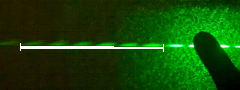
\includegraphics[width=\textwidth]{figuras/medidas/cabelo.pdf}}
  \begin{picture}(\wd\tempbox,\ht\tempbox)
    \put(0,0){\usebox{\tempbox}}
    \put(.36\wd\tempbox,.40\ht\tempbox){\color{white} $3~\Delta y$}
  \end{picture}
\endgroup

\begin{table}[H]
	\centering
	\sisetup{
        round-precision = 5,
        minimum-integer-digits = 2
	}
	\begin{tabular}{cc}
		\toprule\toprule
            {\bfseries Medida} & {\bfseries Valor}
        \\\midrule
        $n_y$           & $3$ \\
        $n_y \Delta y$  & $\SI{101.6(3)}{\milli\meter}$ \\
        $\Delta y$      & $\SI{33.9(1)}{\milli\meter}$ \\
        $b$             & $\SI{57.9(2)}{\micro\meter}$
        \\\bottomrule\bottomrule
	\end{tabular}

	\caption{Dados obtidos para o padrão de difração no fio de cabelo}
	\label{tab:difcab}
\end{table}
\begin{figure}[H]
    \centering

    \begin{subfigure}[t]{.3\textwidth}
        \centering
        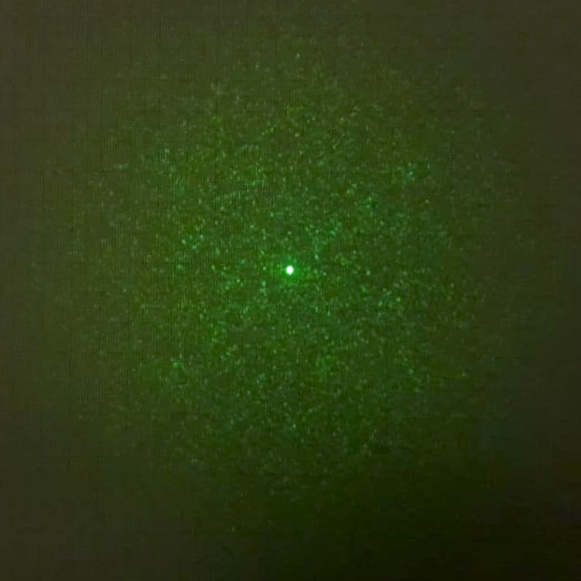
\includegraphics[width=\textwidth]{figuras/medidas/D1.jpg}
        \caption{D1}
        \label{fig:D1}
    \end{subfigure}
    \qquad
    \begin{subfigure}[t]{.3\textwidth}
        \centering
        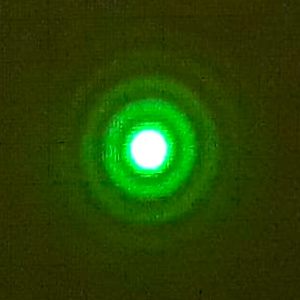
\includegraphics[width=\textwidth]{figuras/medidas/D2.jpg}
        \caption{D2}
        \label{fig:D2}
    \end{subfigure}
    \qquad
    \begin{subfigure}[t]{.3\textwidth}
        \centering
        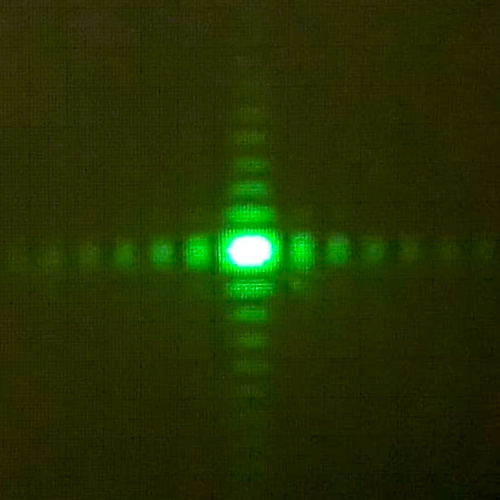
\includegraphics[width=\textwidth]{figuras/medidas/D3.jpg}
        \caption{D3}
        \label{fig:D3}
    \end{subfigure}
    \qquad
    \begin{subfigure}[t]{.3\textwidth}
        \centering
        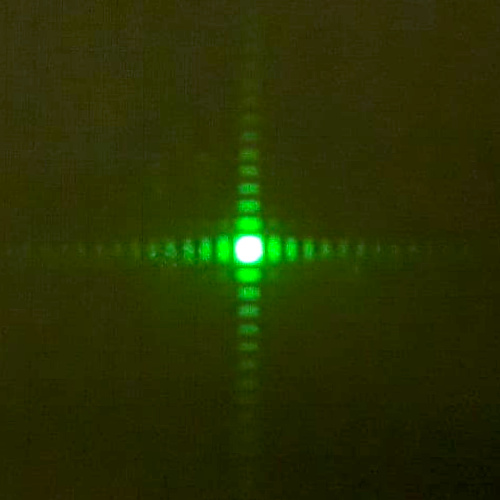
\includegraphics[width=\textwidth]{figuras/medidas/D4.jpg}
        \caption{D4}
        \label{fig:D4}
    \end{subfigure}
    \qquad
    \begin{subfigure}[t]{.3\textwidth}
        \centering
        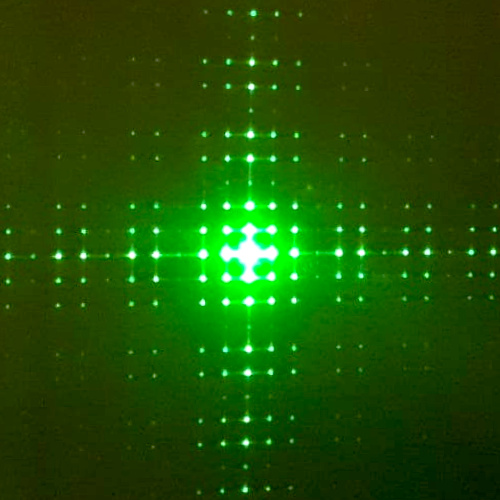
\includegraphics[width=\textwidth]{figuras/medidas/D5.jpg}
        \caption{D5}
        \label{fig:D5}
    \end{subfigure}
    \qquad
    \begin{subfigure}[t]{.3\textwidth}
        \centering
        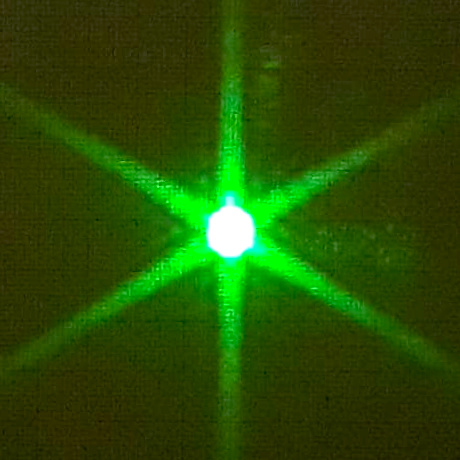
\includegraphics[width=\textwidth]{figuras/medidas/D6.jpg}
        \caption{D6}
        \label{fig:D6}
    \end{subfigure}

    \caption{Fotos dos padrões de difração das fendas D}
    \label{fig:D}
\end{figure}
